\documentclass[11pt]{article}
\usepackage{graphicx} % Required for inserting images
\usepackage{amsmath, amssymb, setspace}
\usepackage{hyperref}
\title{Some Cool Plots}
\author{Josh Sack}
\begin{document}
\maketitle 
\listoffigures
\listoftables
\begin{figure}
    \centering
    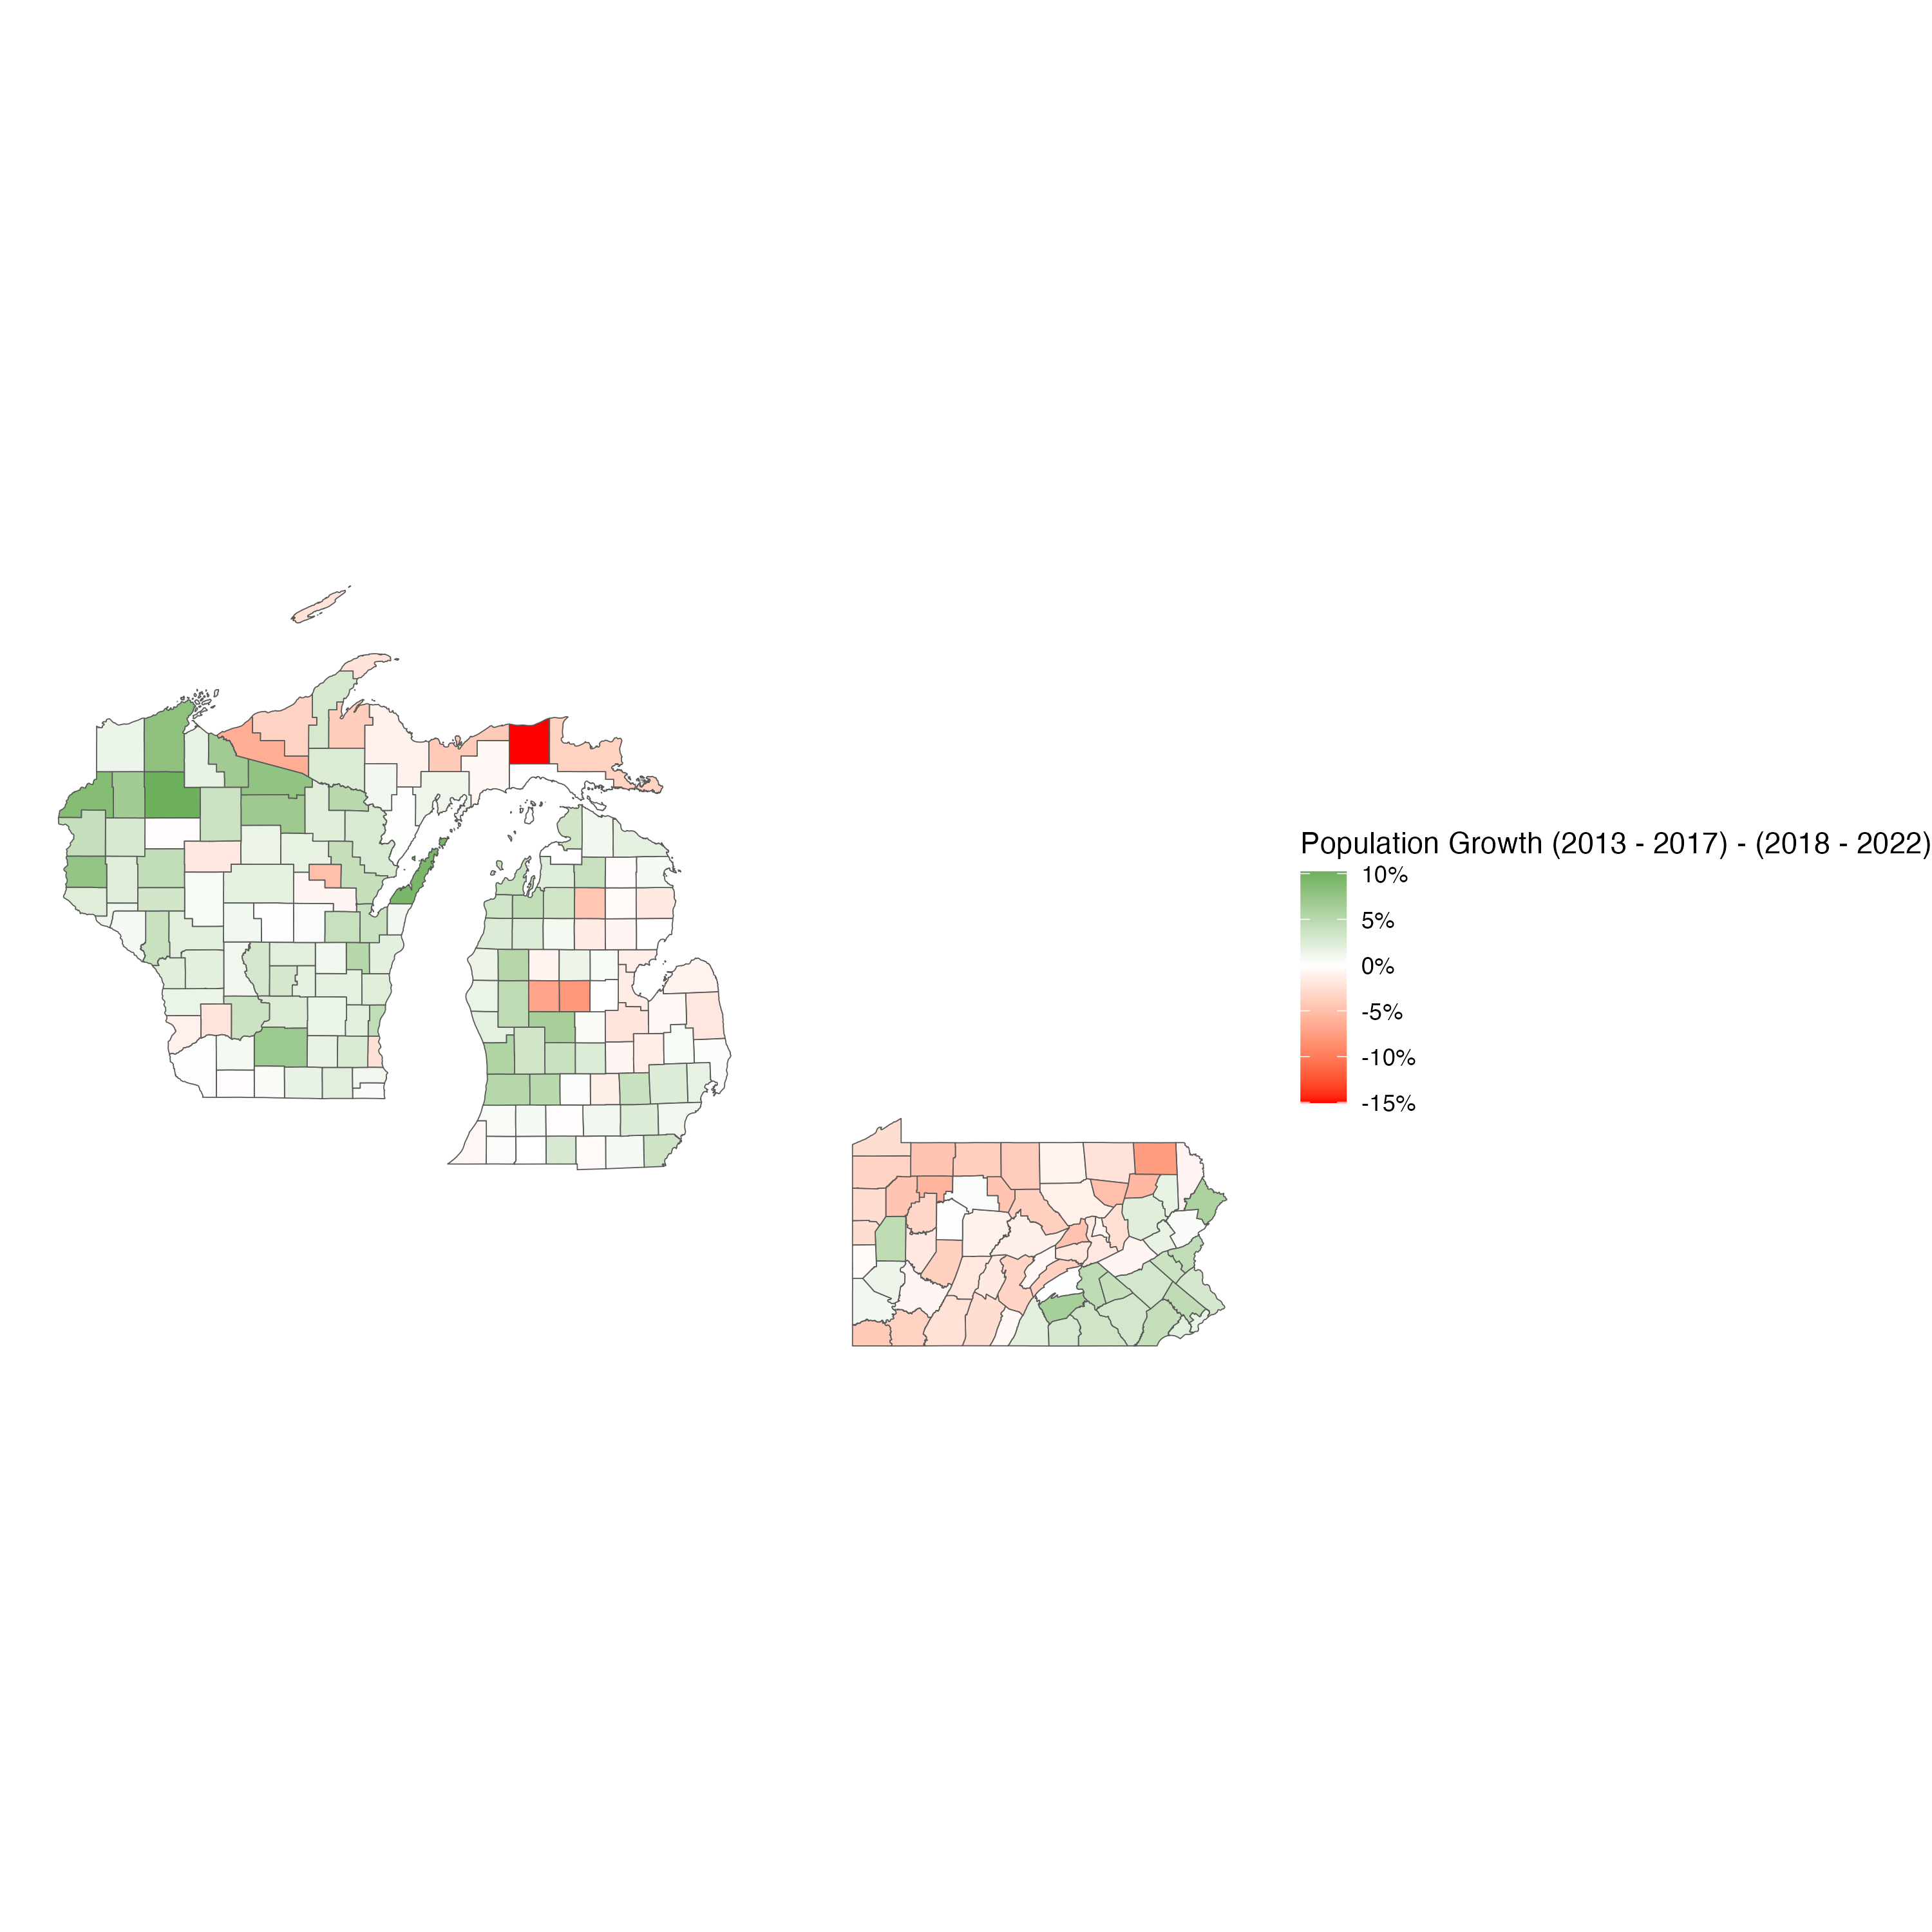
\includegraphics[width=0.9\textwidth]{plots/blue-wall-growth.png}
    \caption{The population growth rate of counties in the blue wall states from the 2017 ACS to the 2022 ACS}
\end{figure}
\begin{figure}
    \centering 
    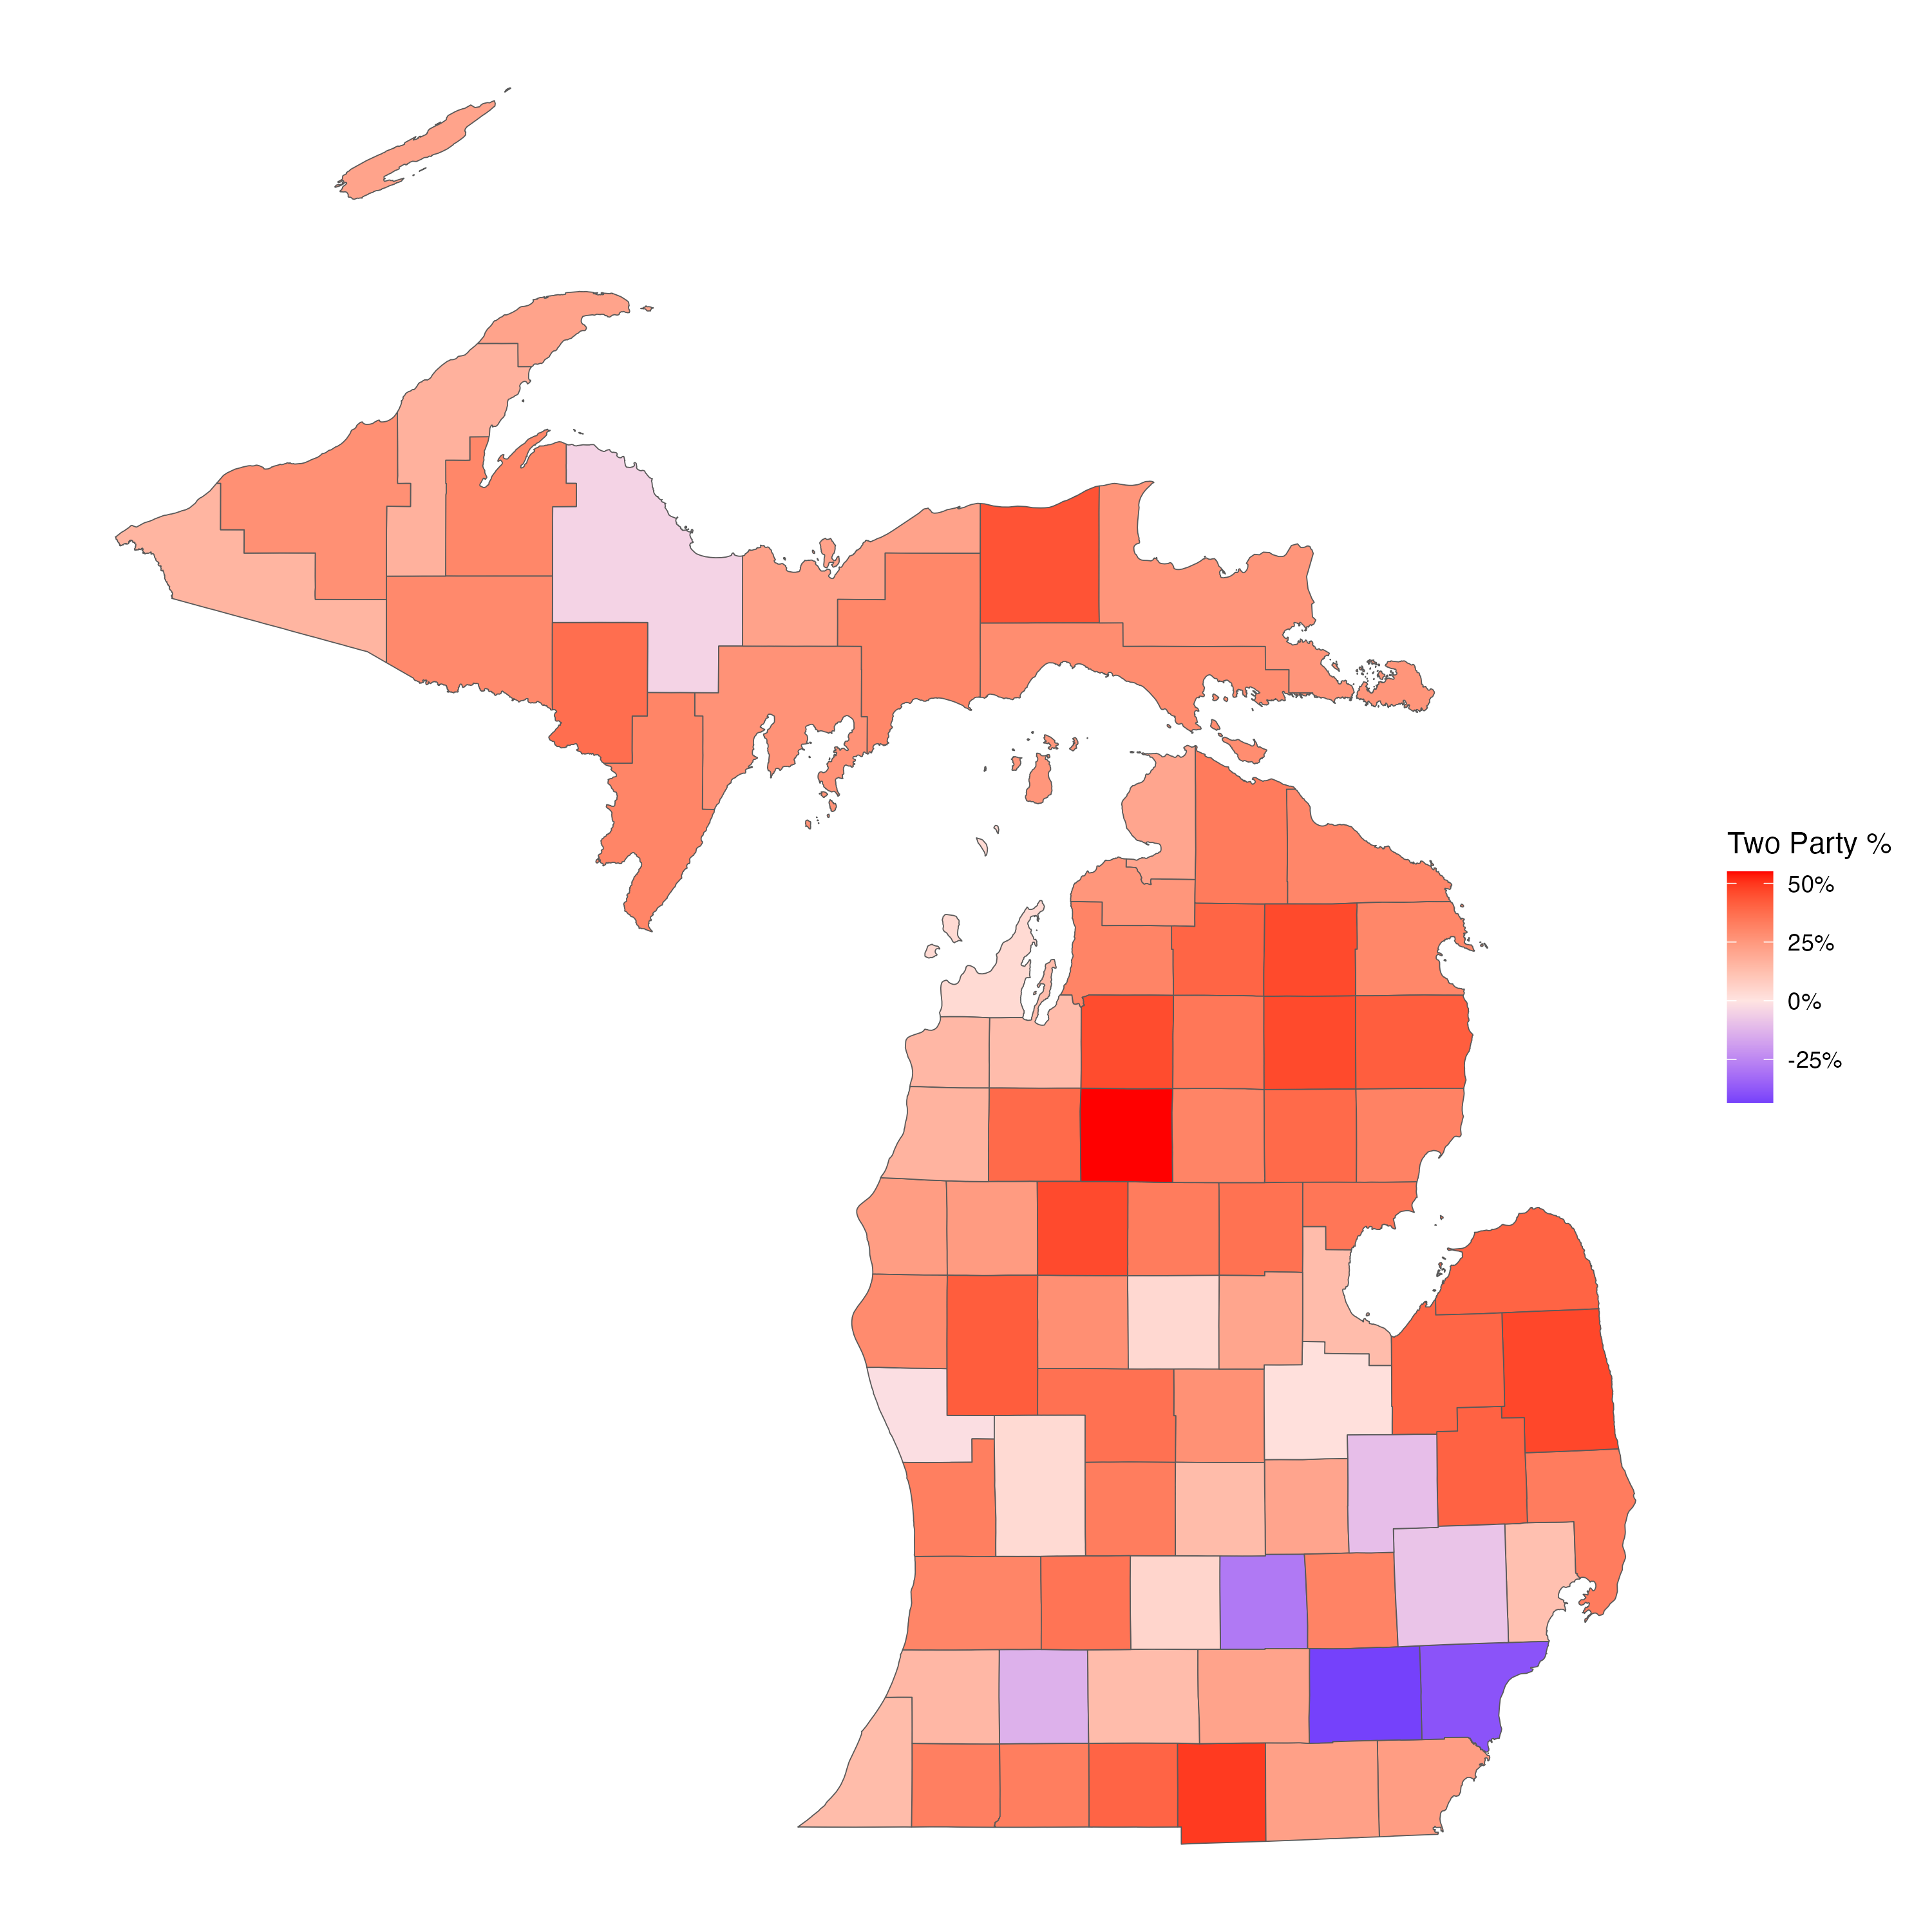
\includegraphics[width=0.9\textwidth]{plots/county-results.png}
    \caption{Michigan: 2016 Presidential Election Results by County}
    \label{fig:2016-results}
\end{figure}
\begin{figure}
    \centering
    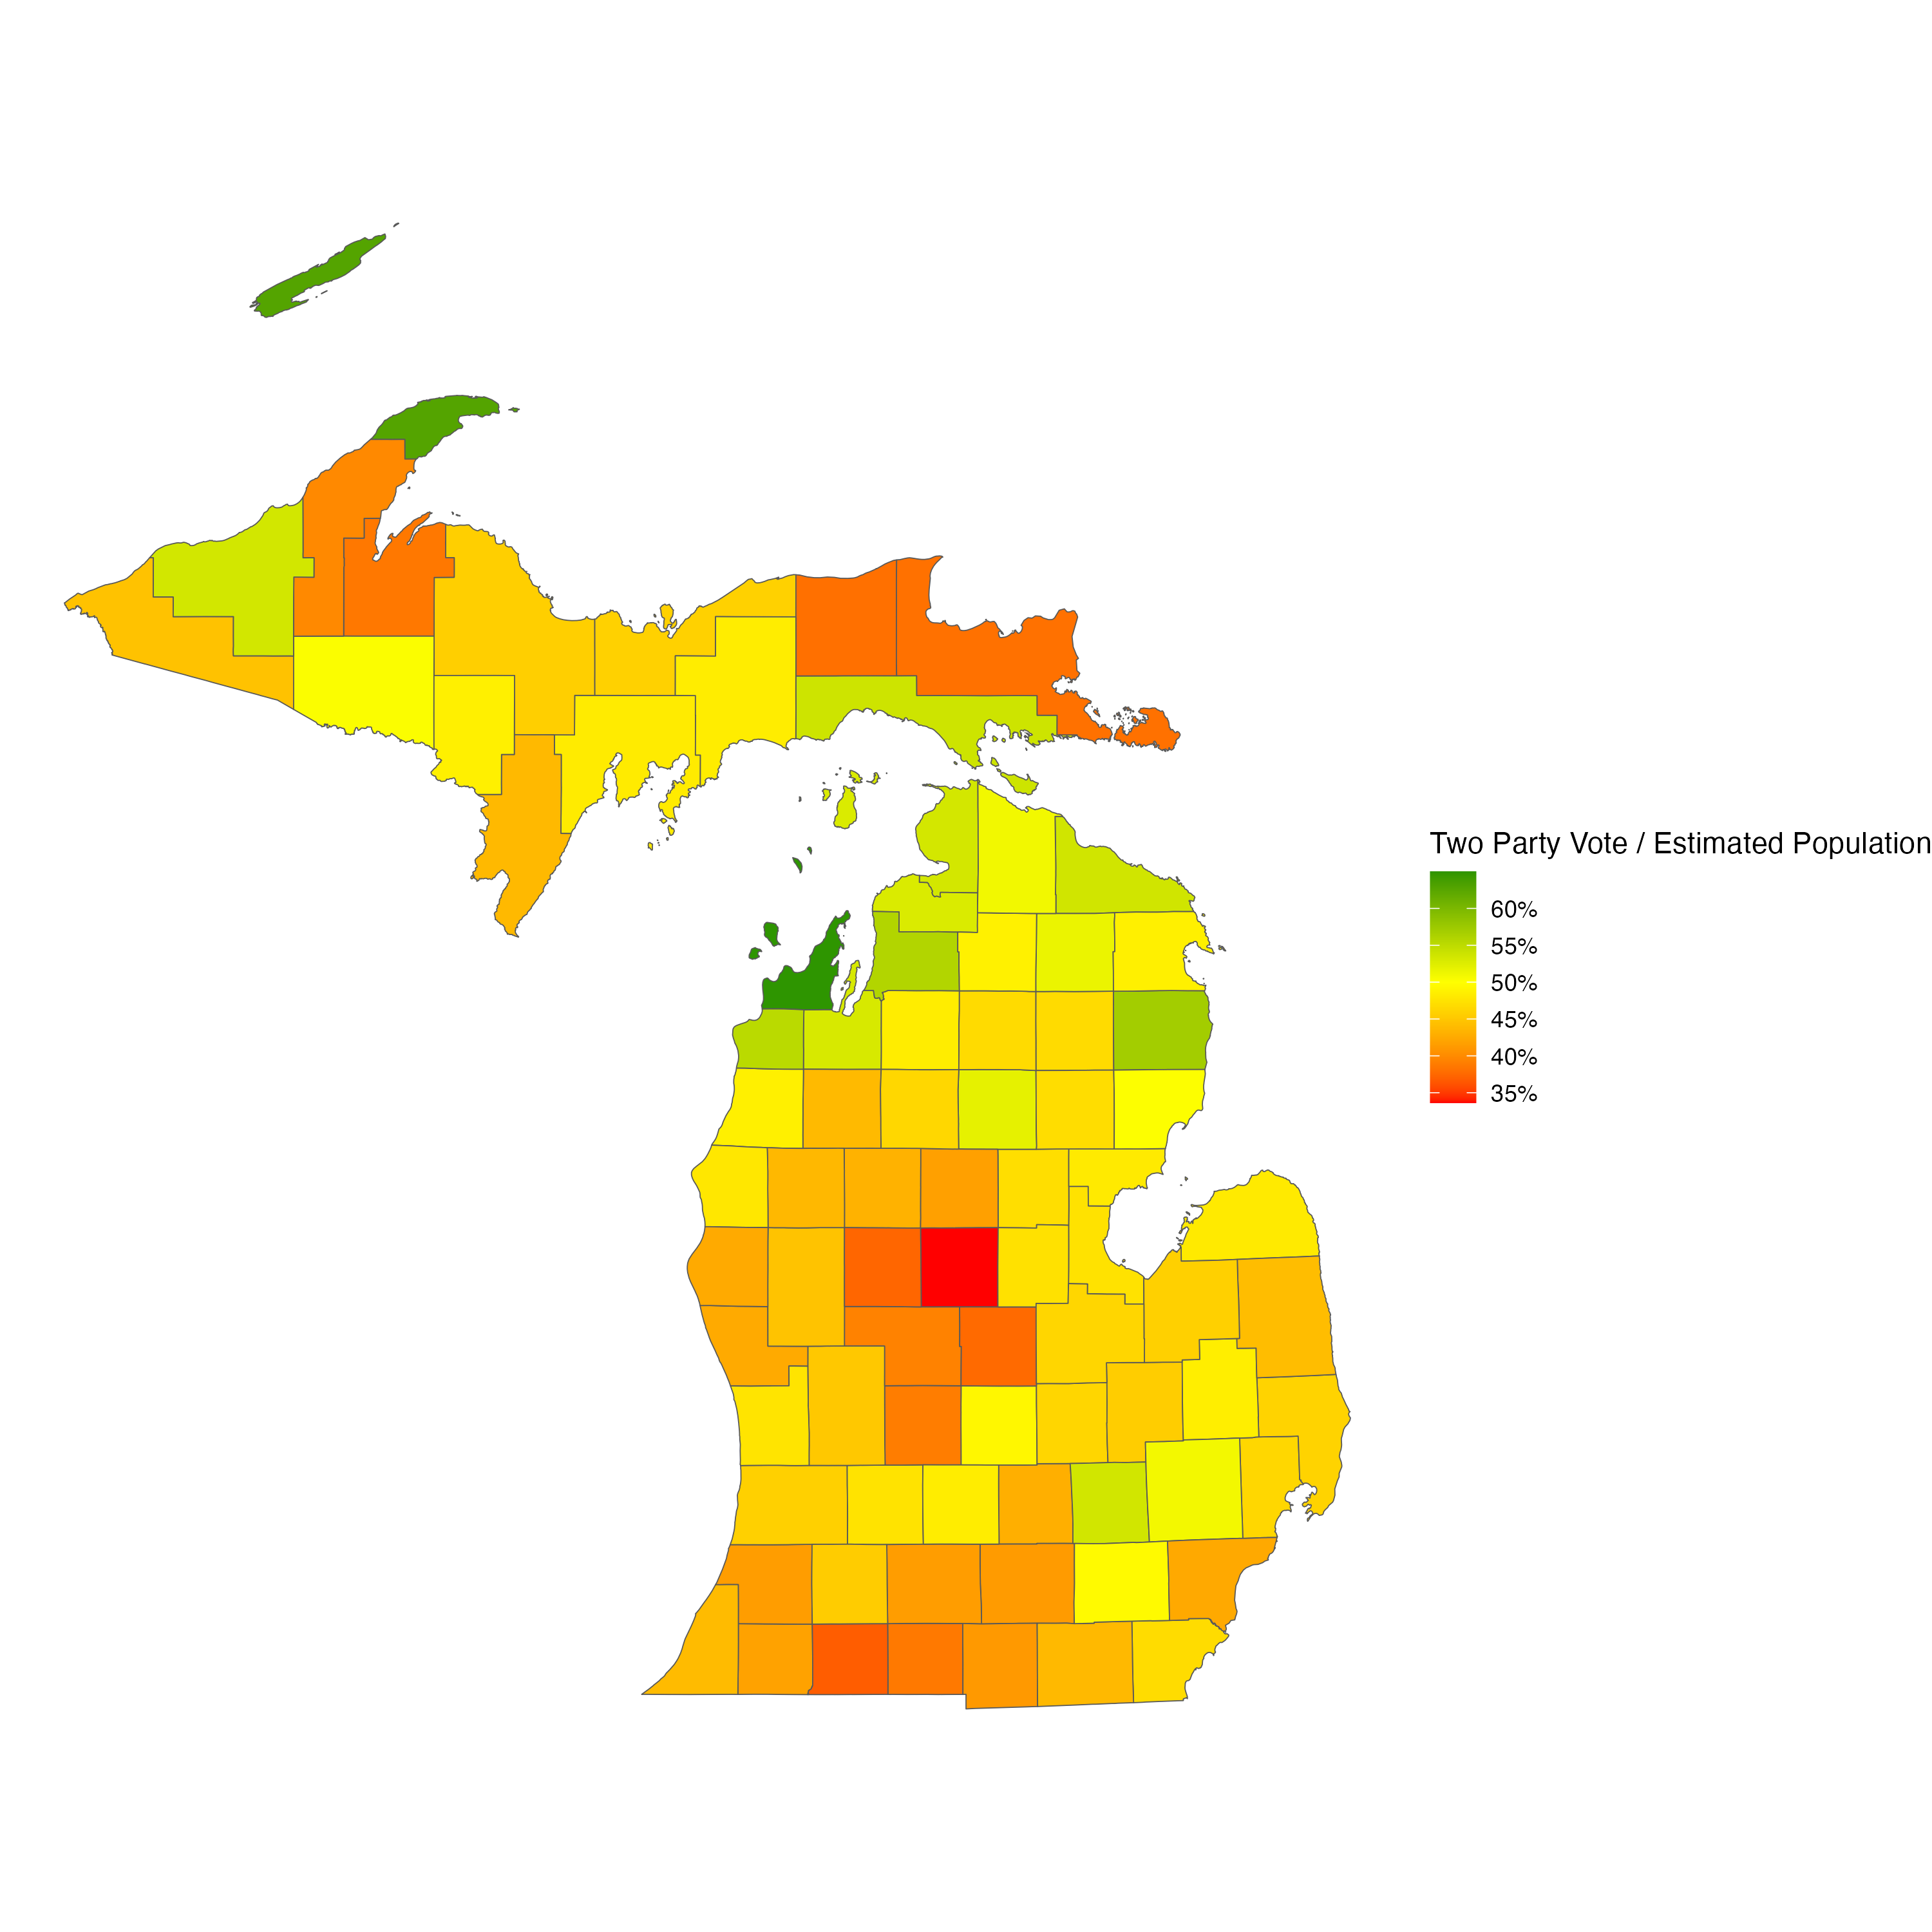
\includegraphics[width=0.9\textwidth]{plots/turnout.png}
    \caption{Michigan: Each County's Two Party Vote as a Percentage of its estimated population in the 2013-2017 American Community Survey}
    \label{fig:turnout}
\end{figure}
\begin{figure}
    \centering
    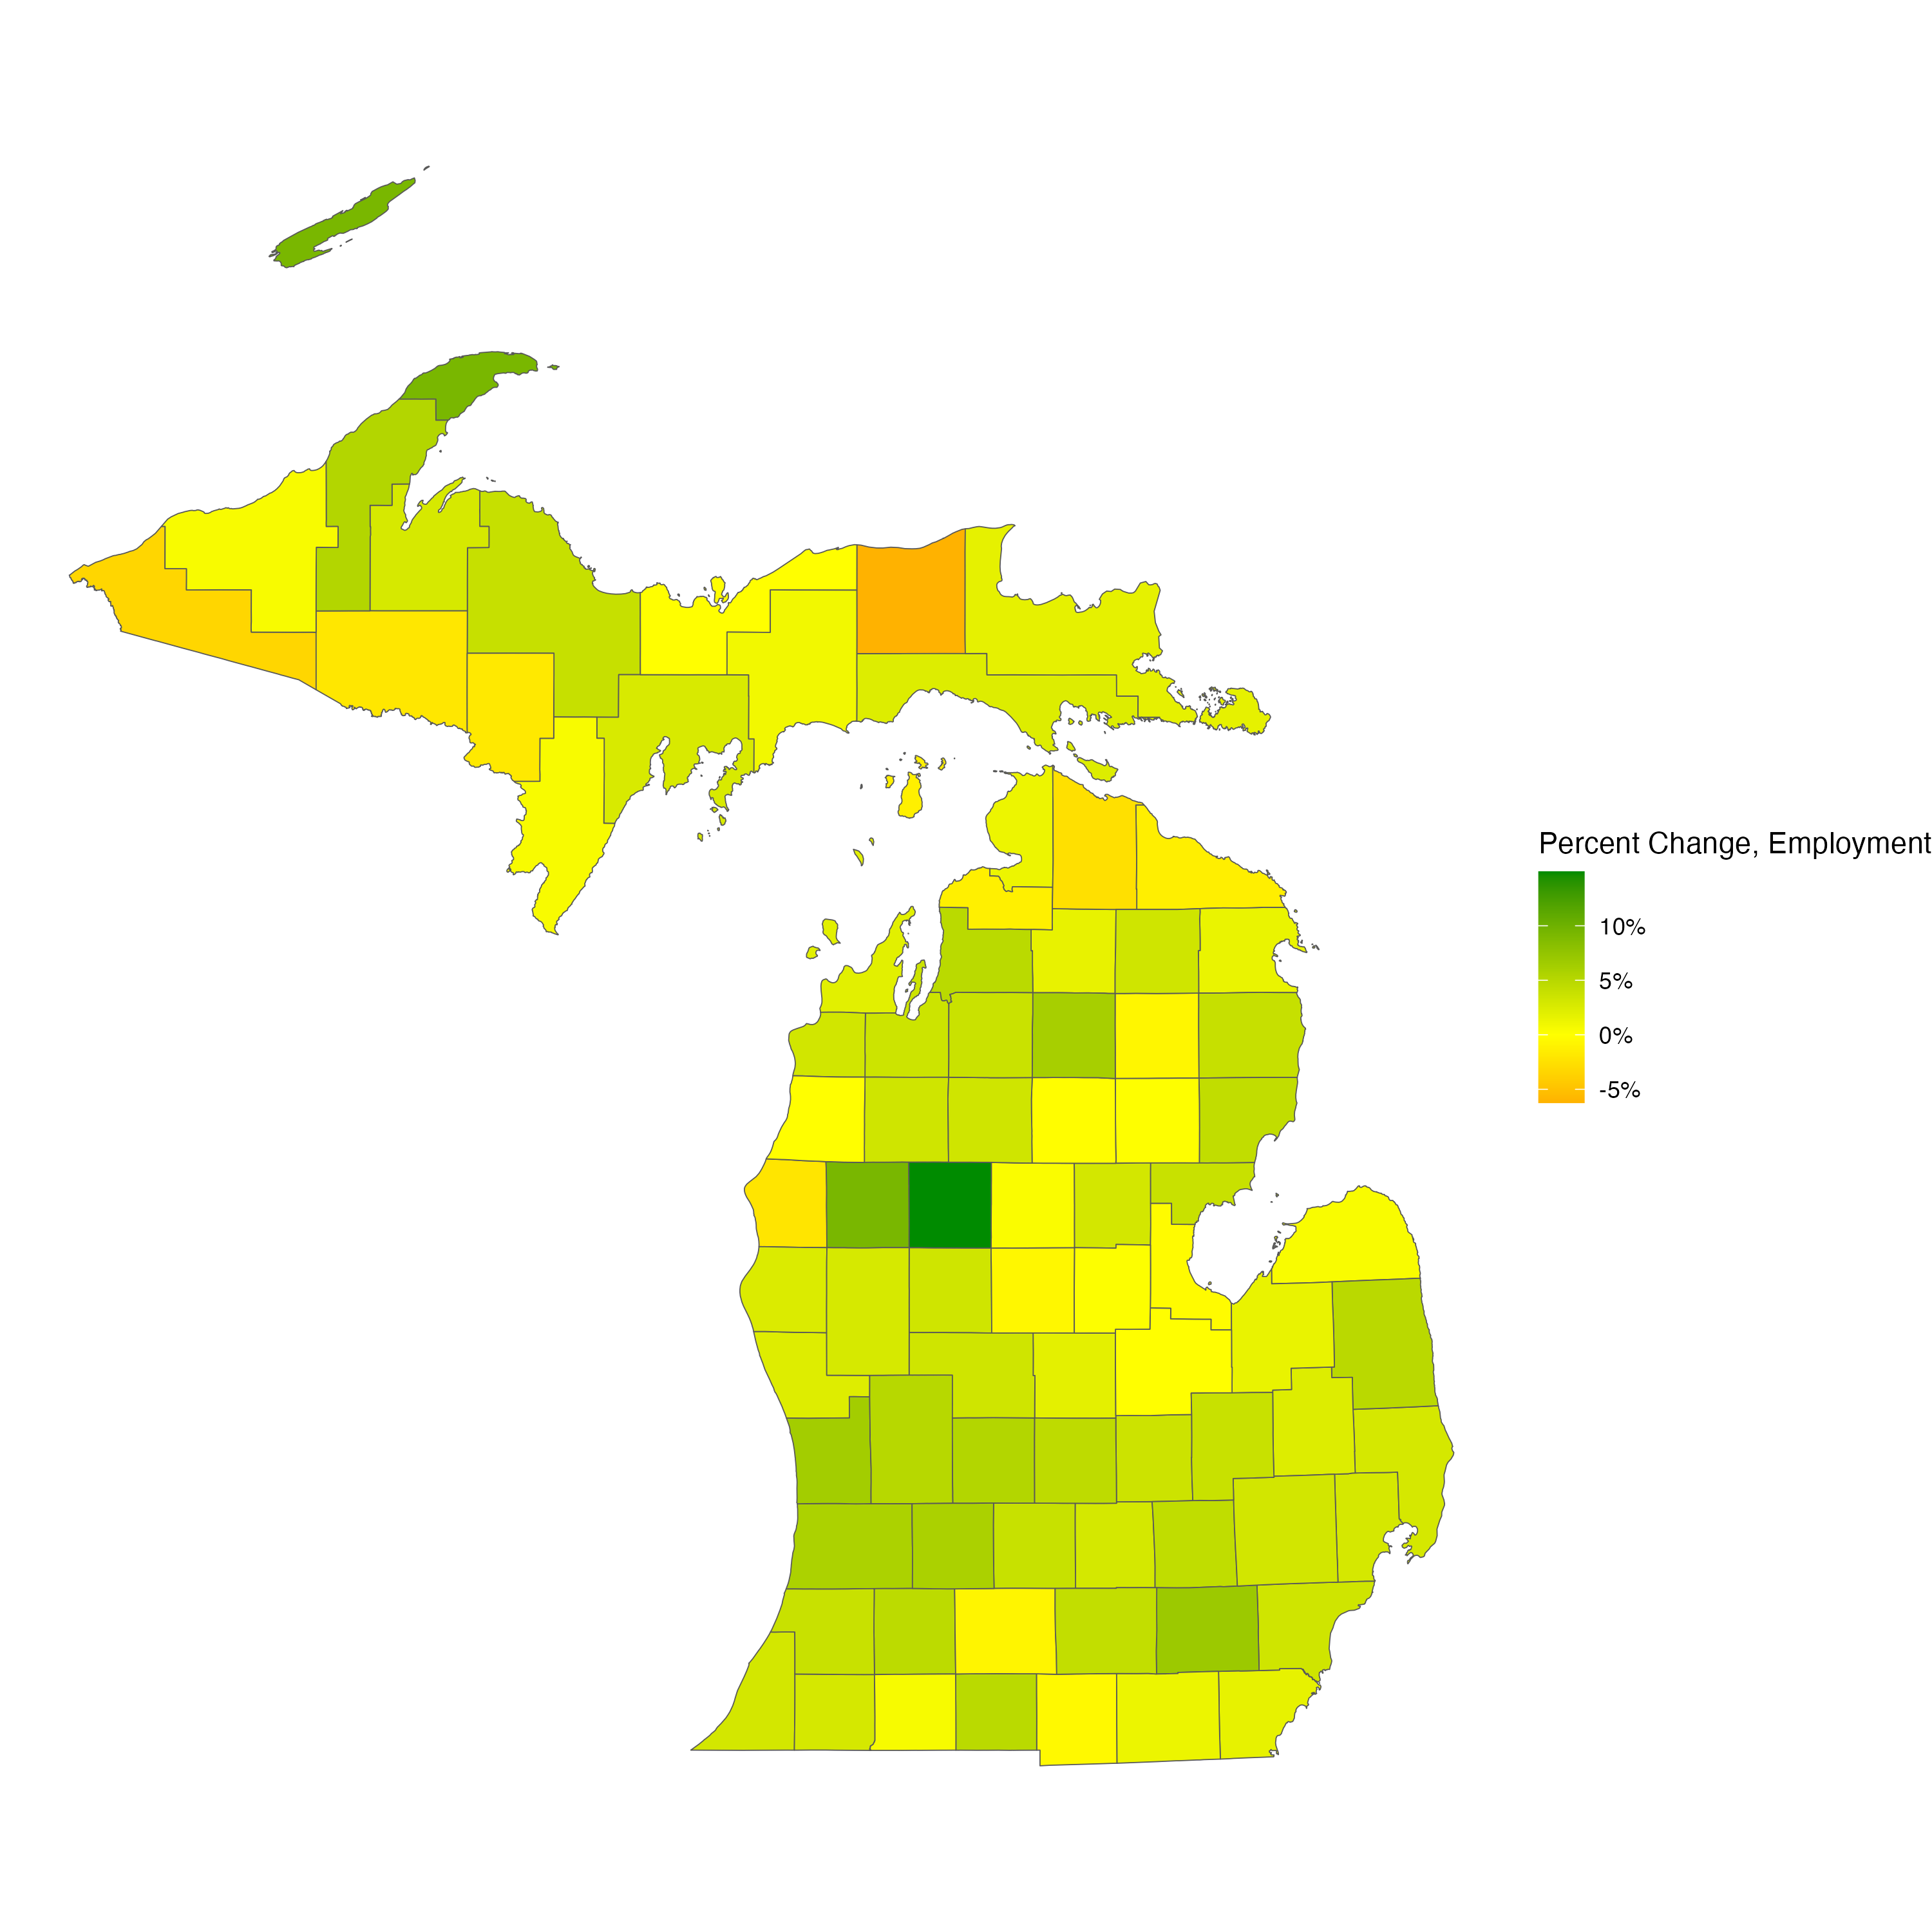
\includegraphics[width=0.9\textwidth]{plots/raw-employment-plot.png}
    \caption{Michigan: The percent change in the number of employed workers in each County from Trump's inauguration to February 2020, the Month before the pandemic hit}
\end{figure}
\begin{figure}
    \centering
    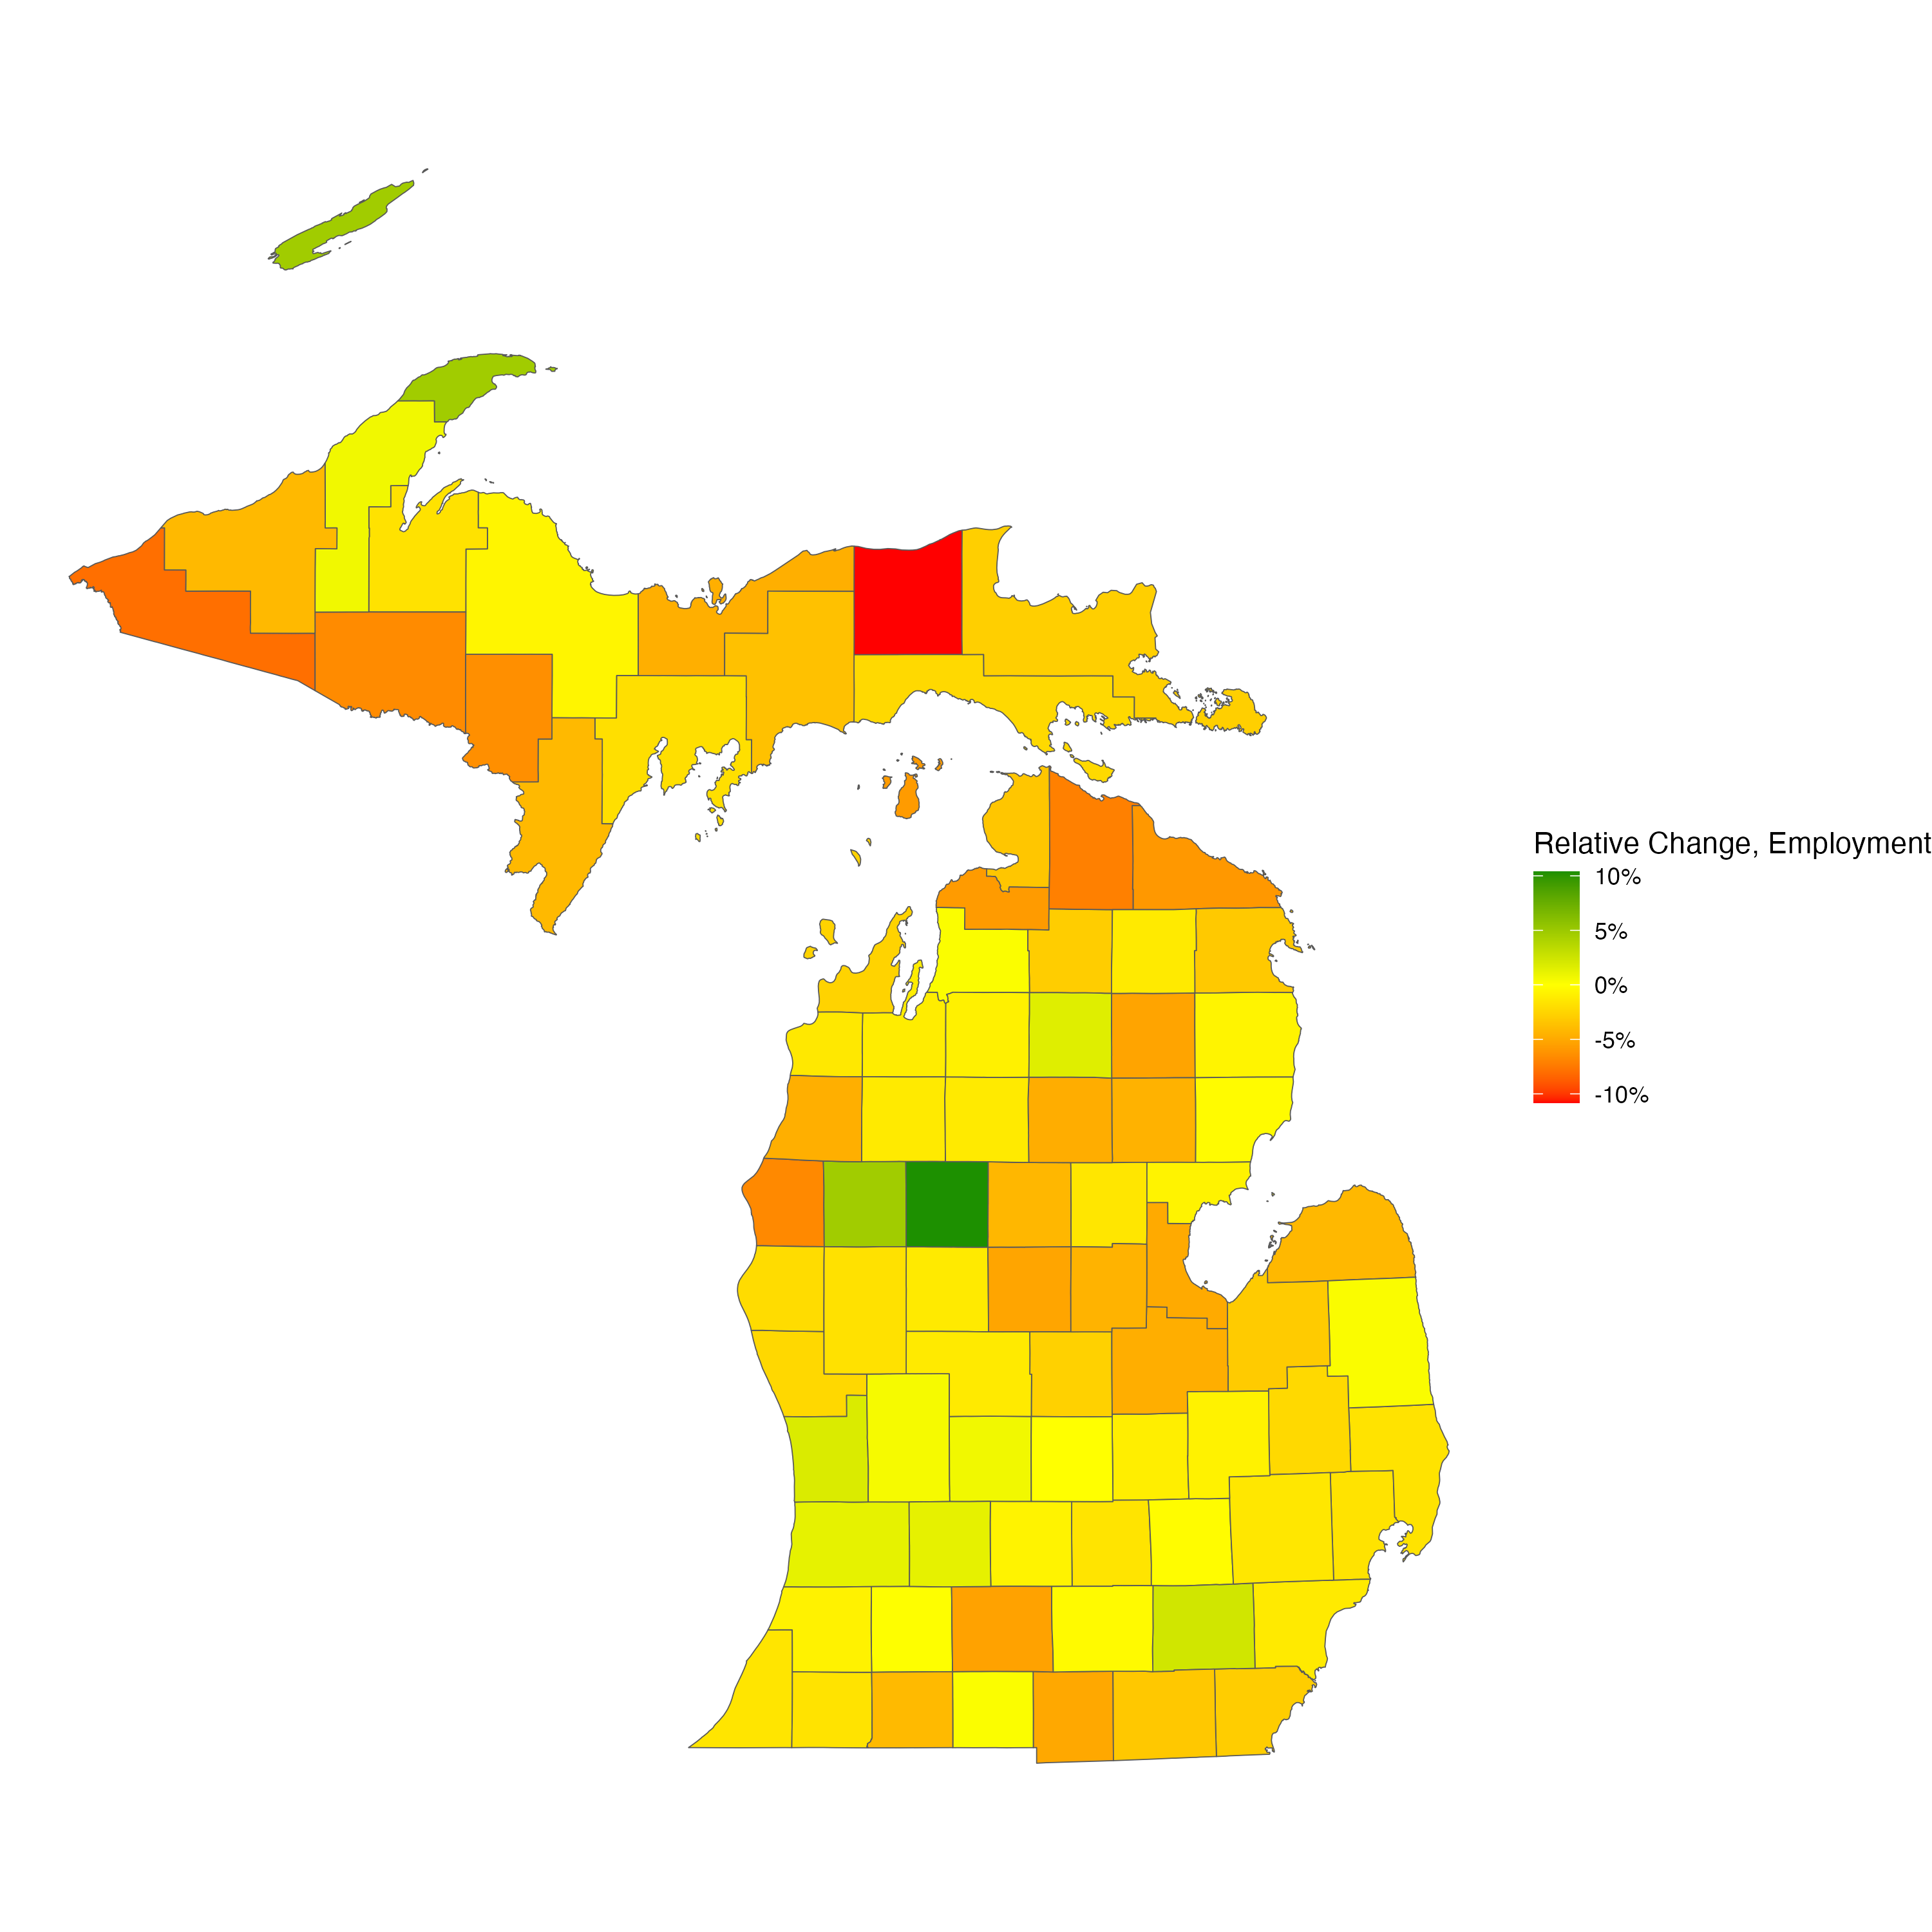
\includegraphics[width=0.9\textwidth]{plots/relative-employment-plot.png}
    \caption{Michigan: The percent change in the number of employed workers in each county in Michigan minus the national percent change in the number of employed workers over the period from Trump's inauguration to February 2020}
\end{figure}
\begin{figure}
    \centering
    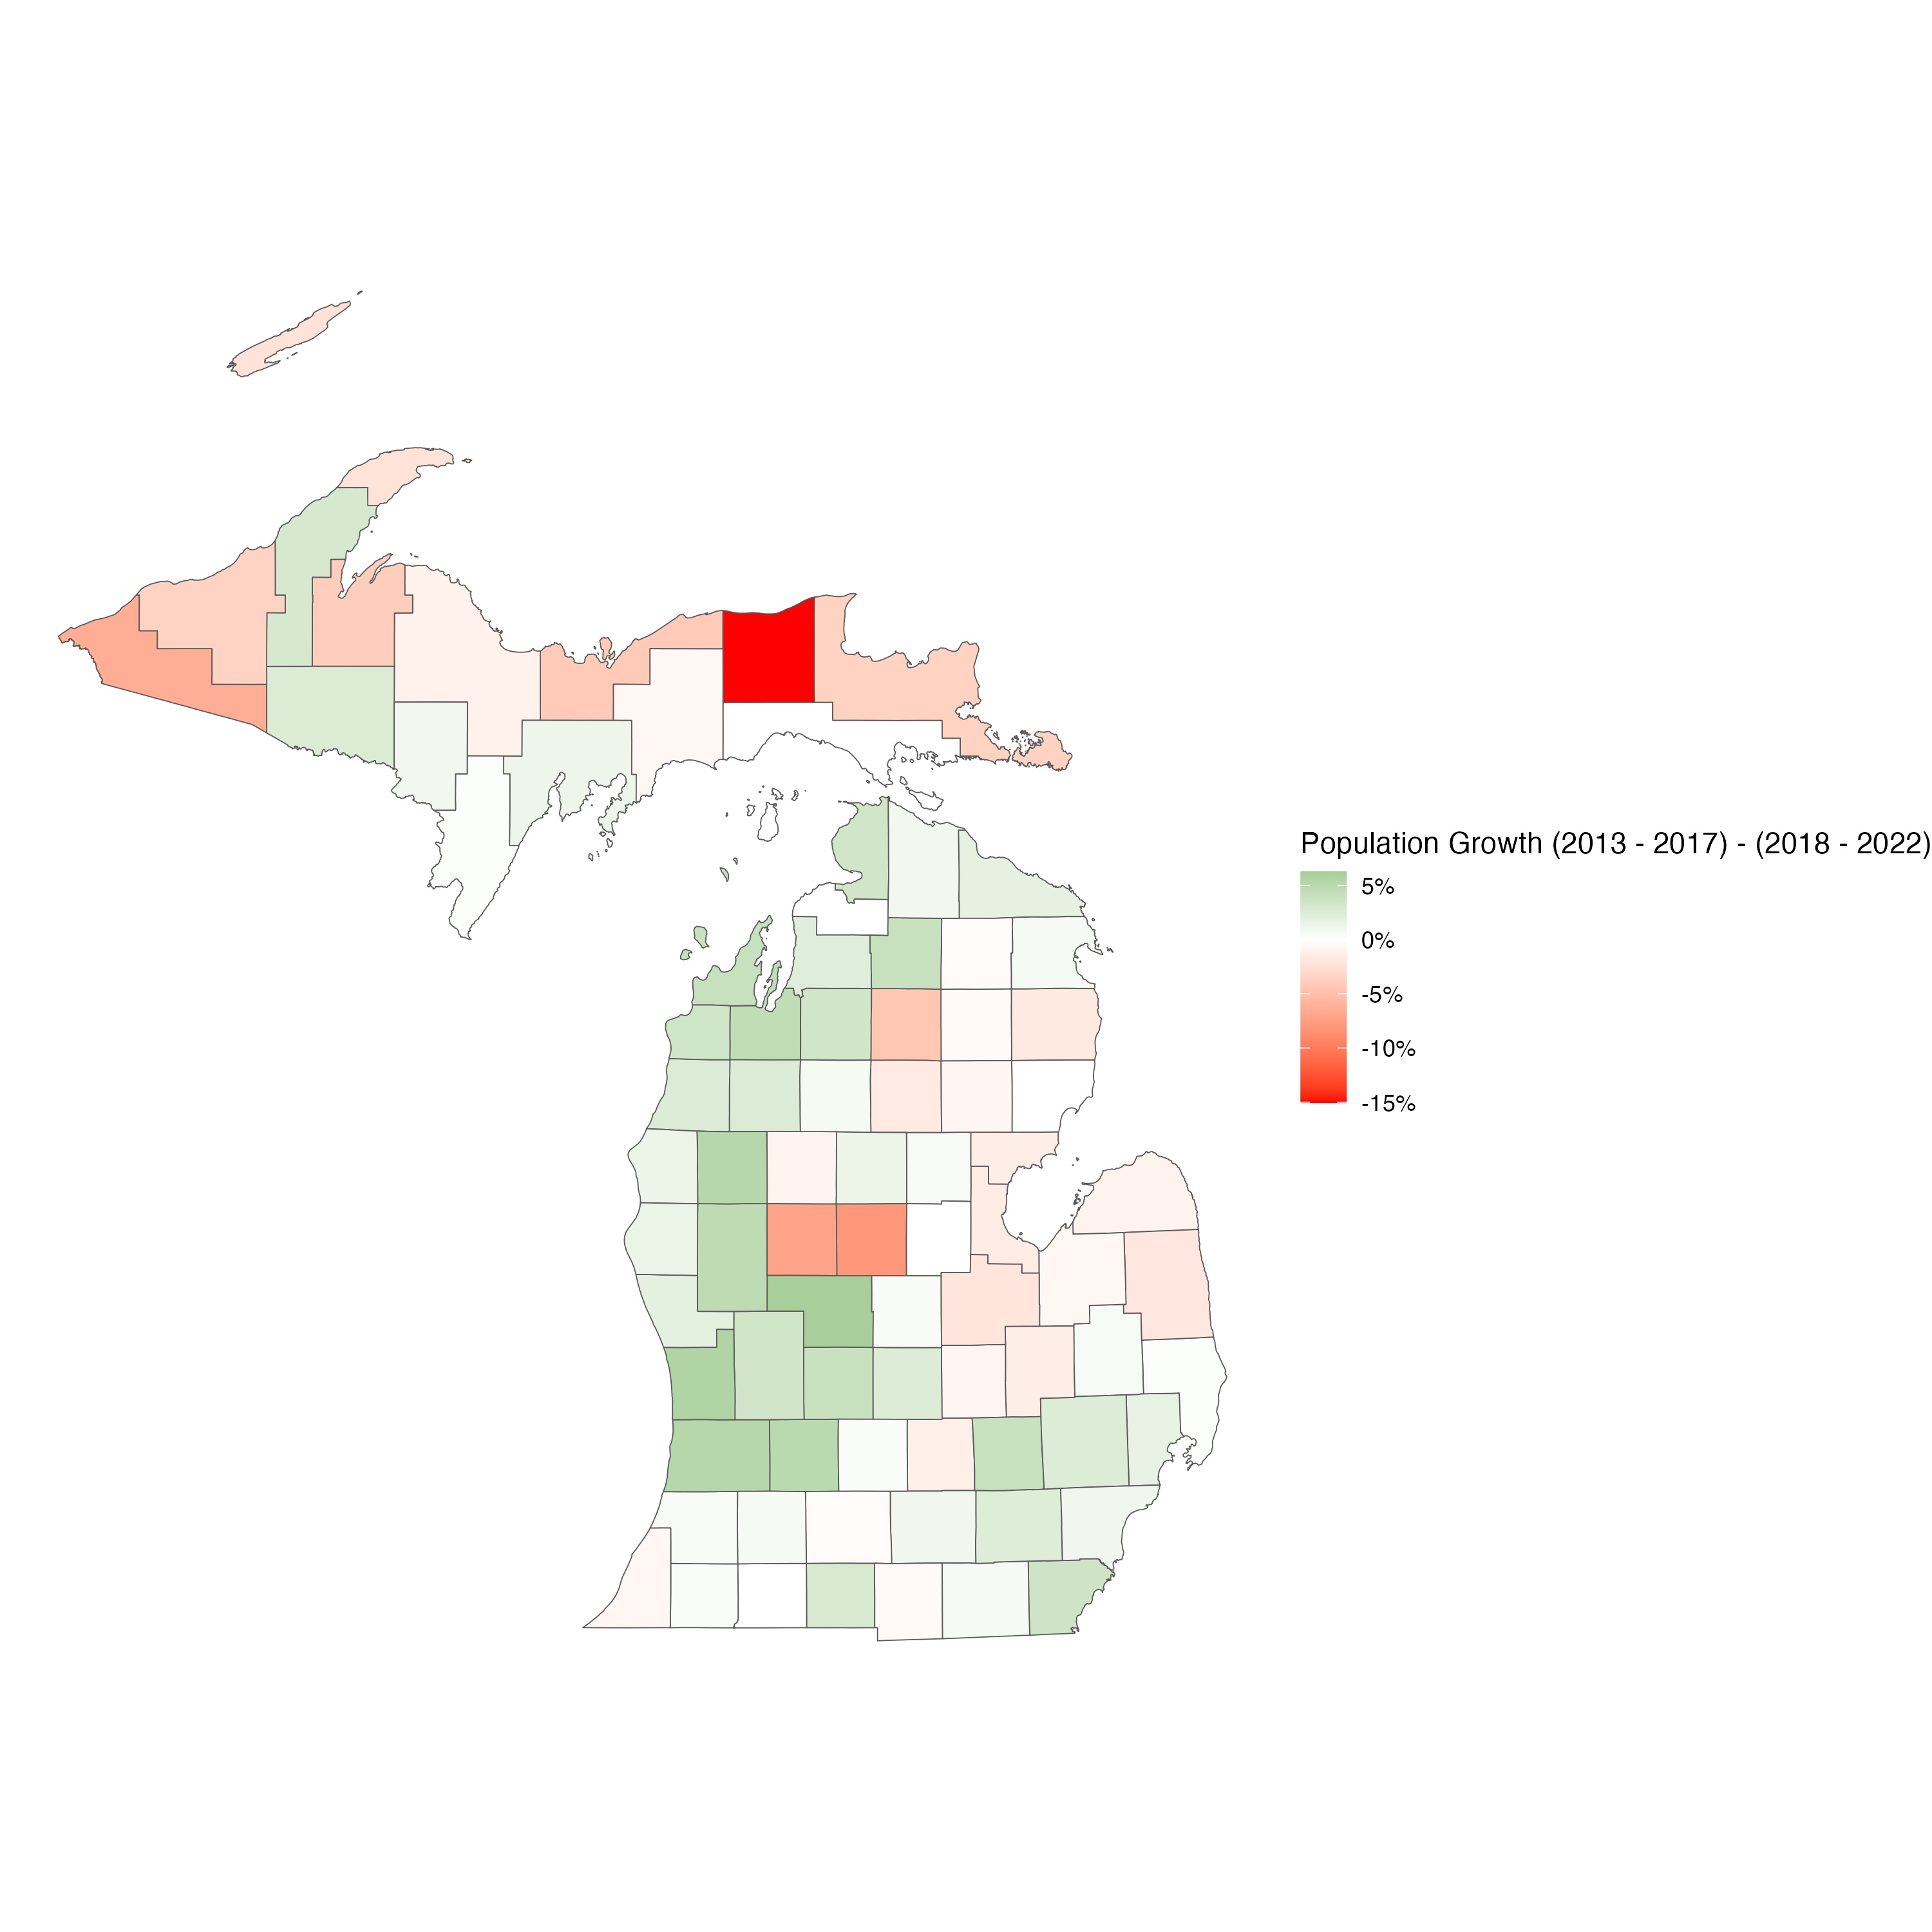
\includegraphics[width=0.9\textwidth]{plots/mi-growth.png}
    \caption{Michigan: County level population growth from the 2017 ACS to the 2022 ACS}
\end{figure}
\begin{figure}
    \centering
    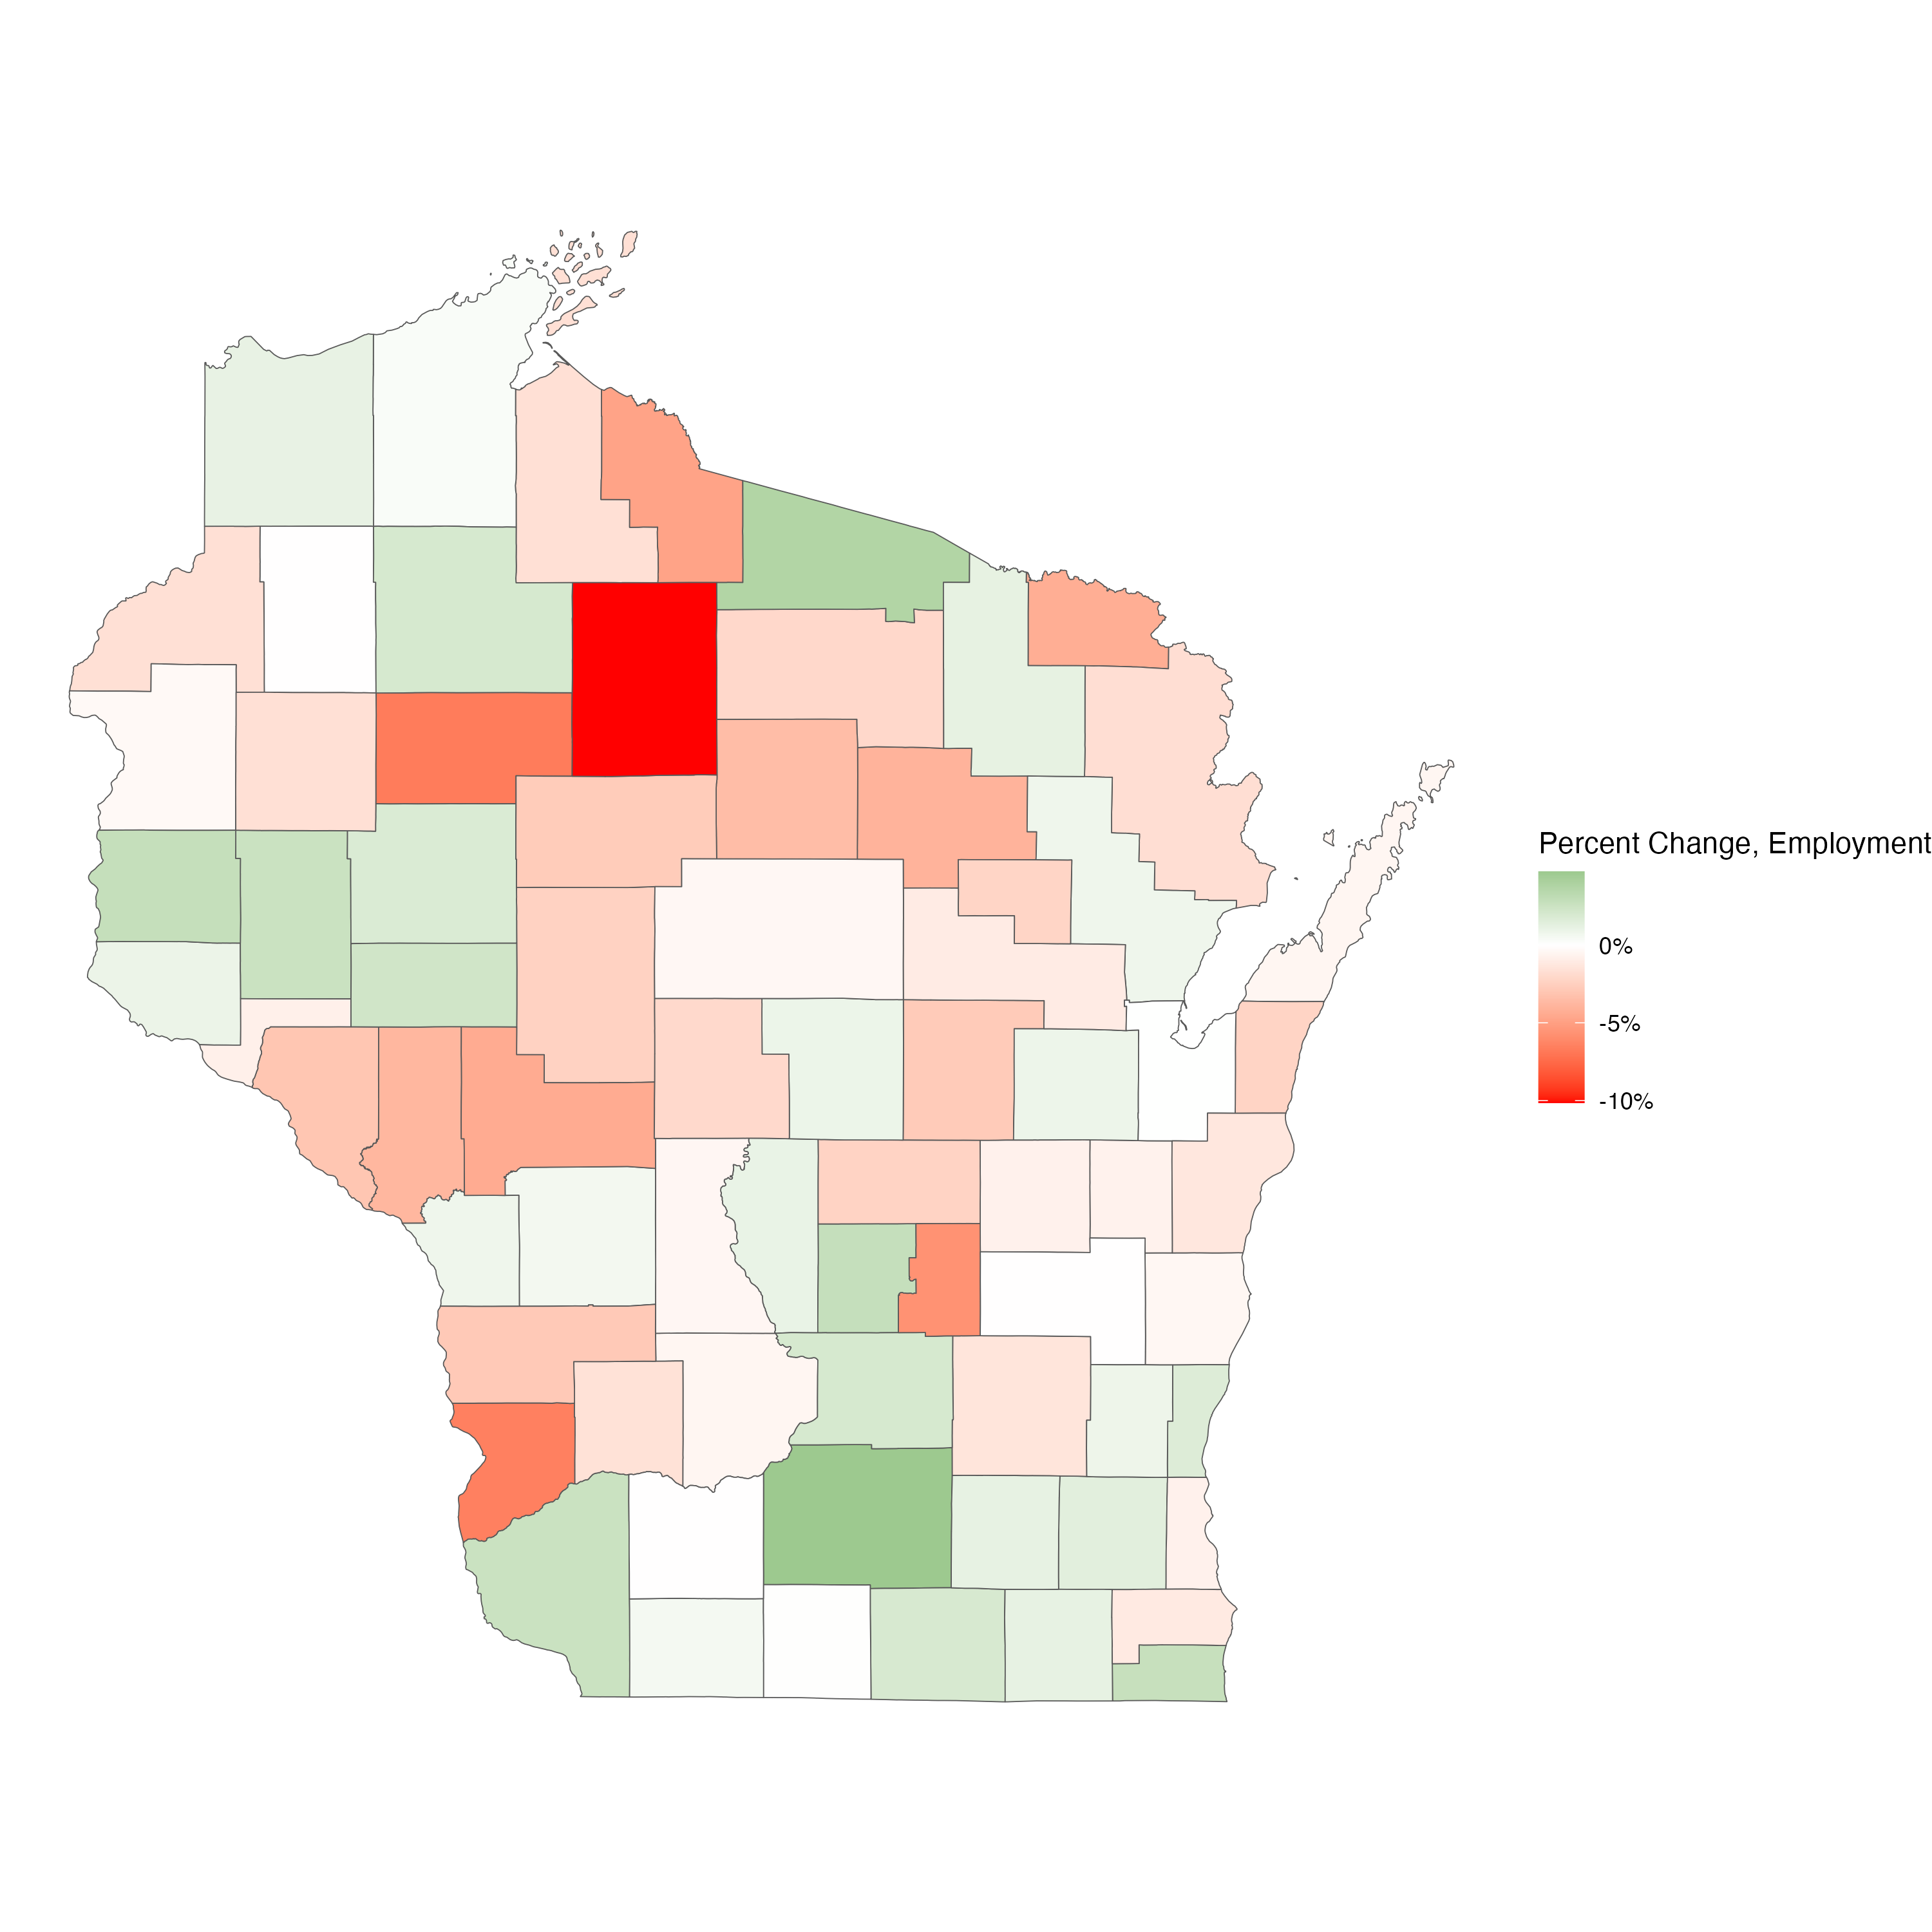
\includegraphics[width=0.9\textwidth]{plots/raw-employment-plot-wi.png}
    \caption{Wisconsin: The percent change in the number of employed workers in each County from Trump's inauguration to February 2020, the Month before the pandemic hit}
\end{figure}
\begin{figure}
    \centering
    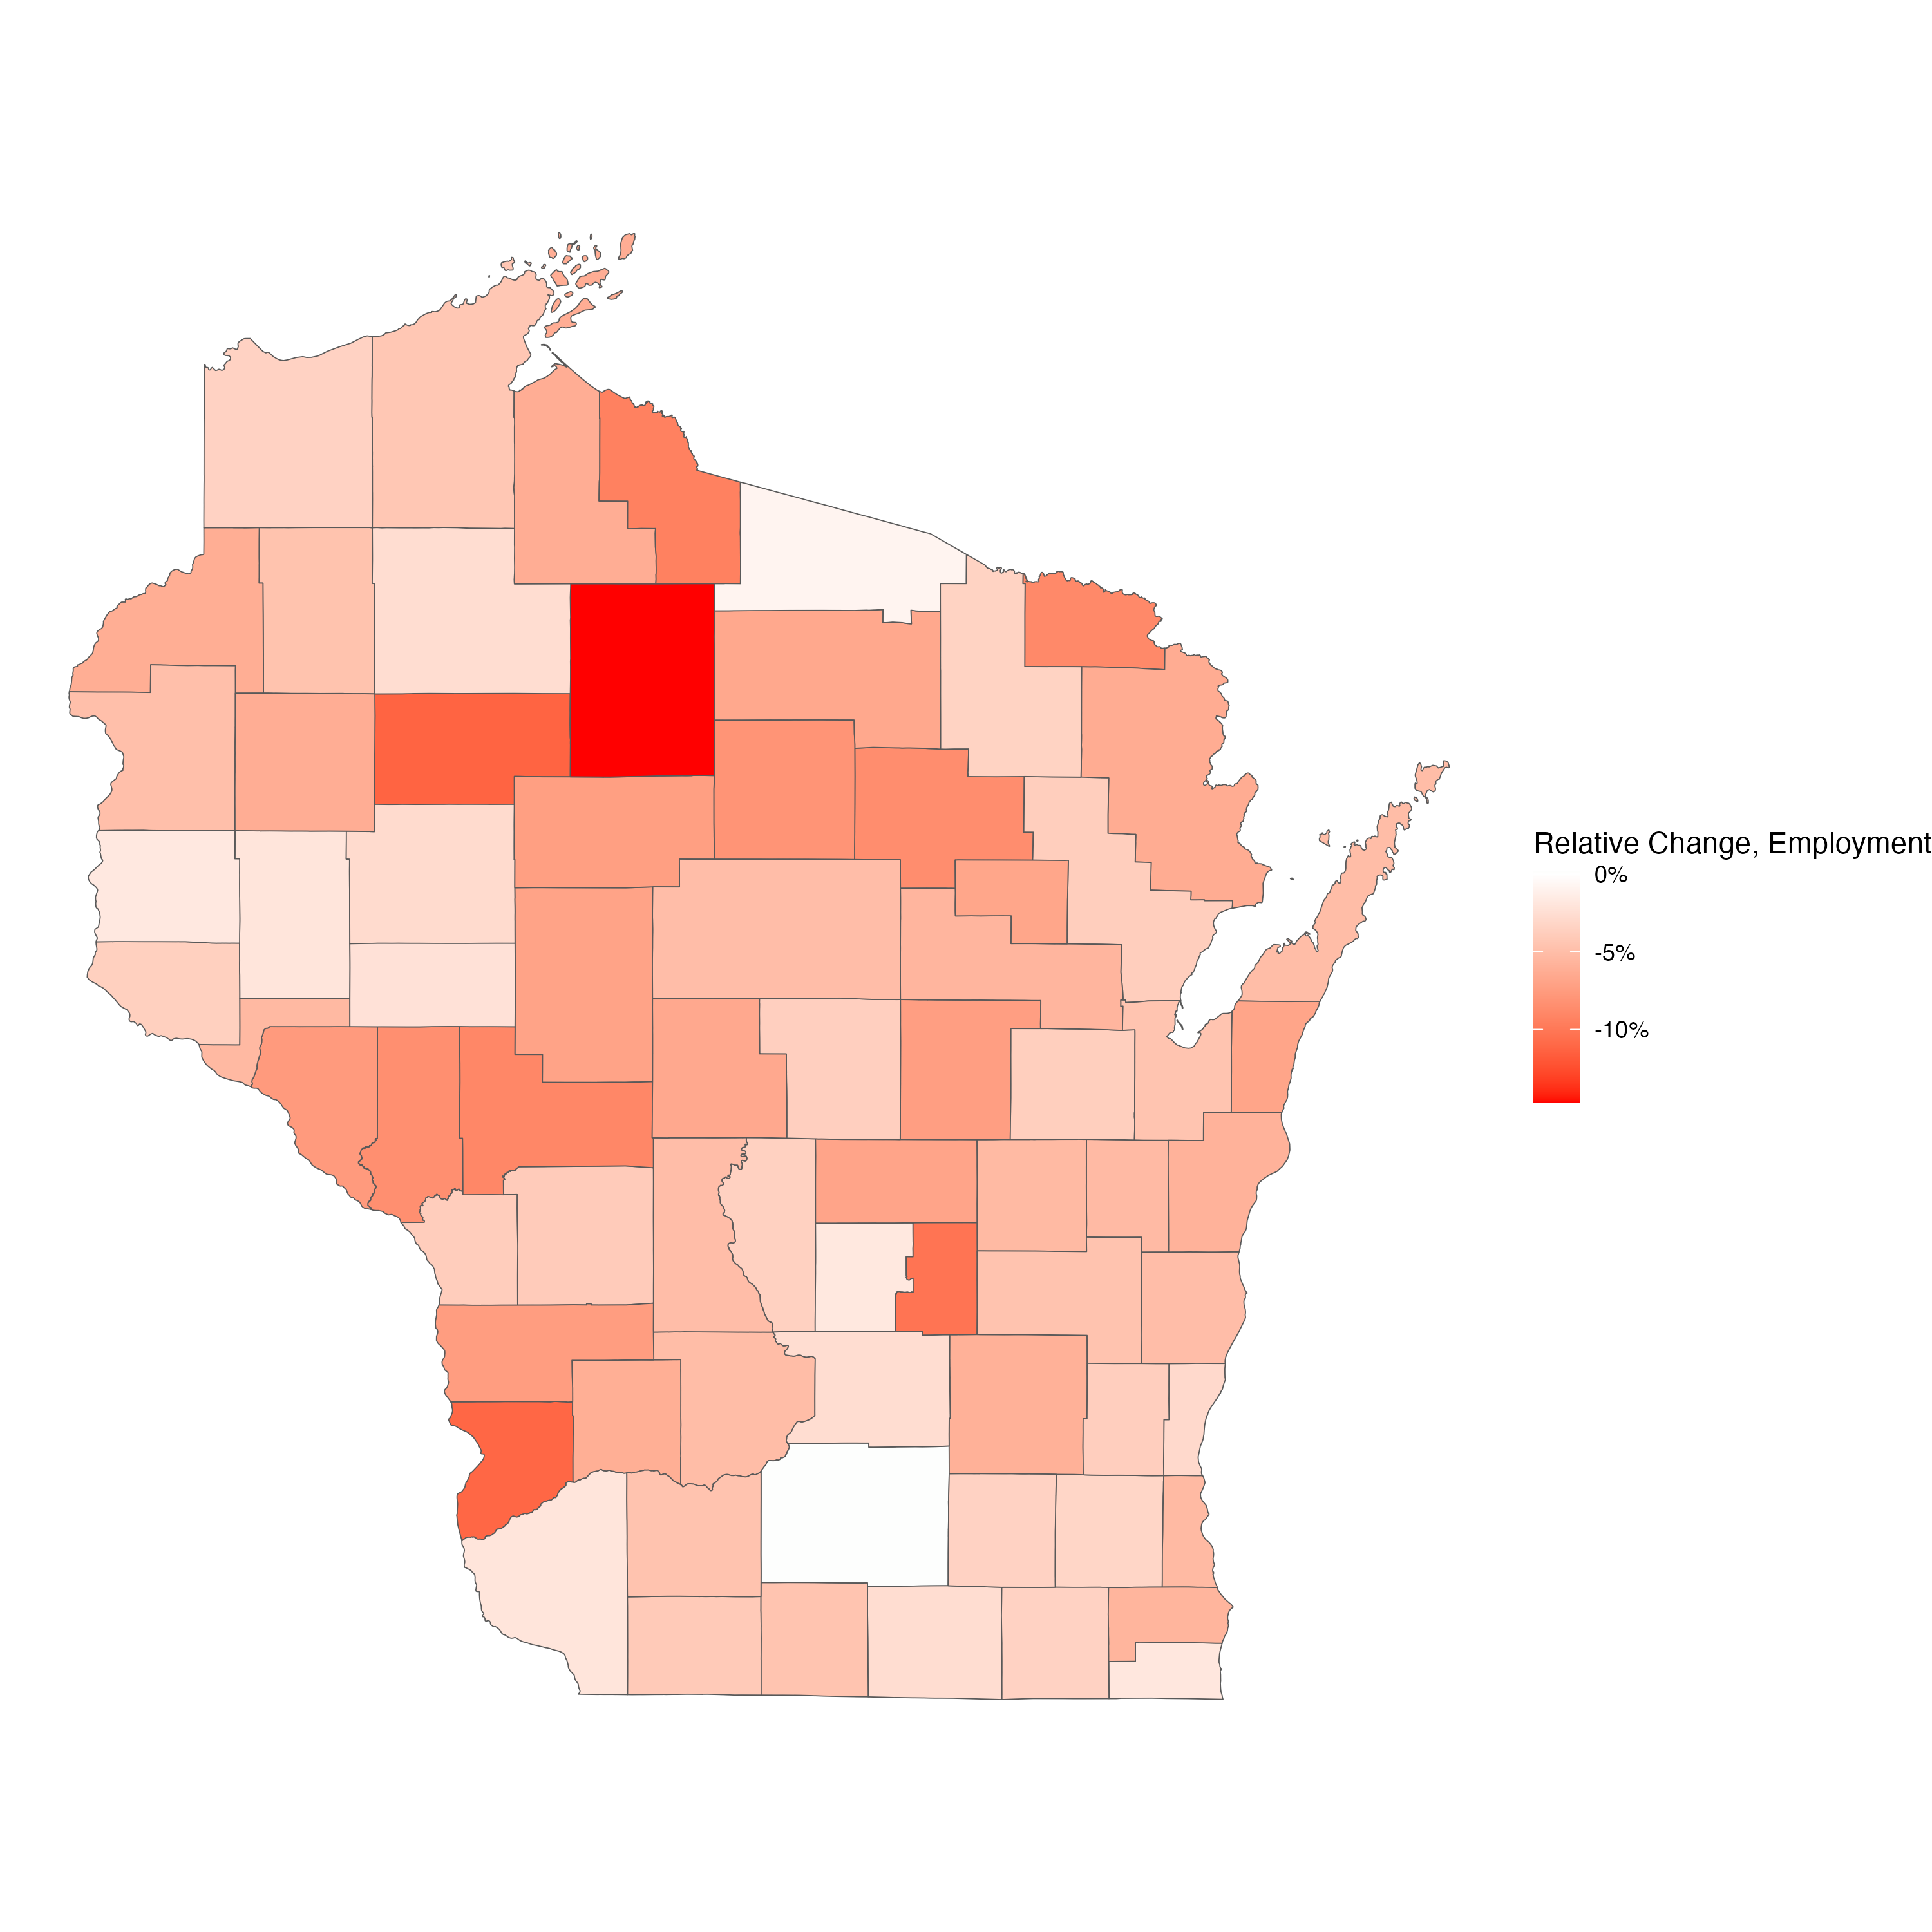
\includegraphics[width=0.9\textwidth]{plots/relative-employment-plot-wi.png}
    \caption{The percent change in the number of employed workers in each county in Wisconsin minus the national percent change in the number of employed workers over the period from Trump's inauguration to February 2020}
\end{figure}
\begin{figure}
    \centering
    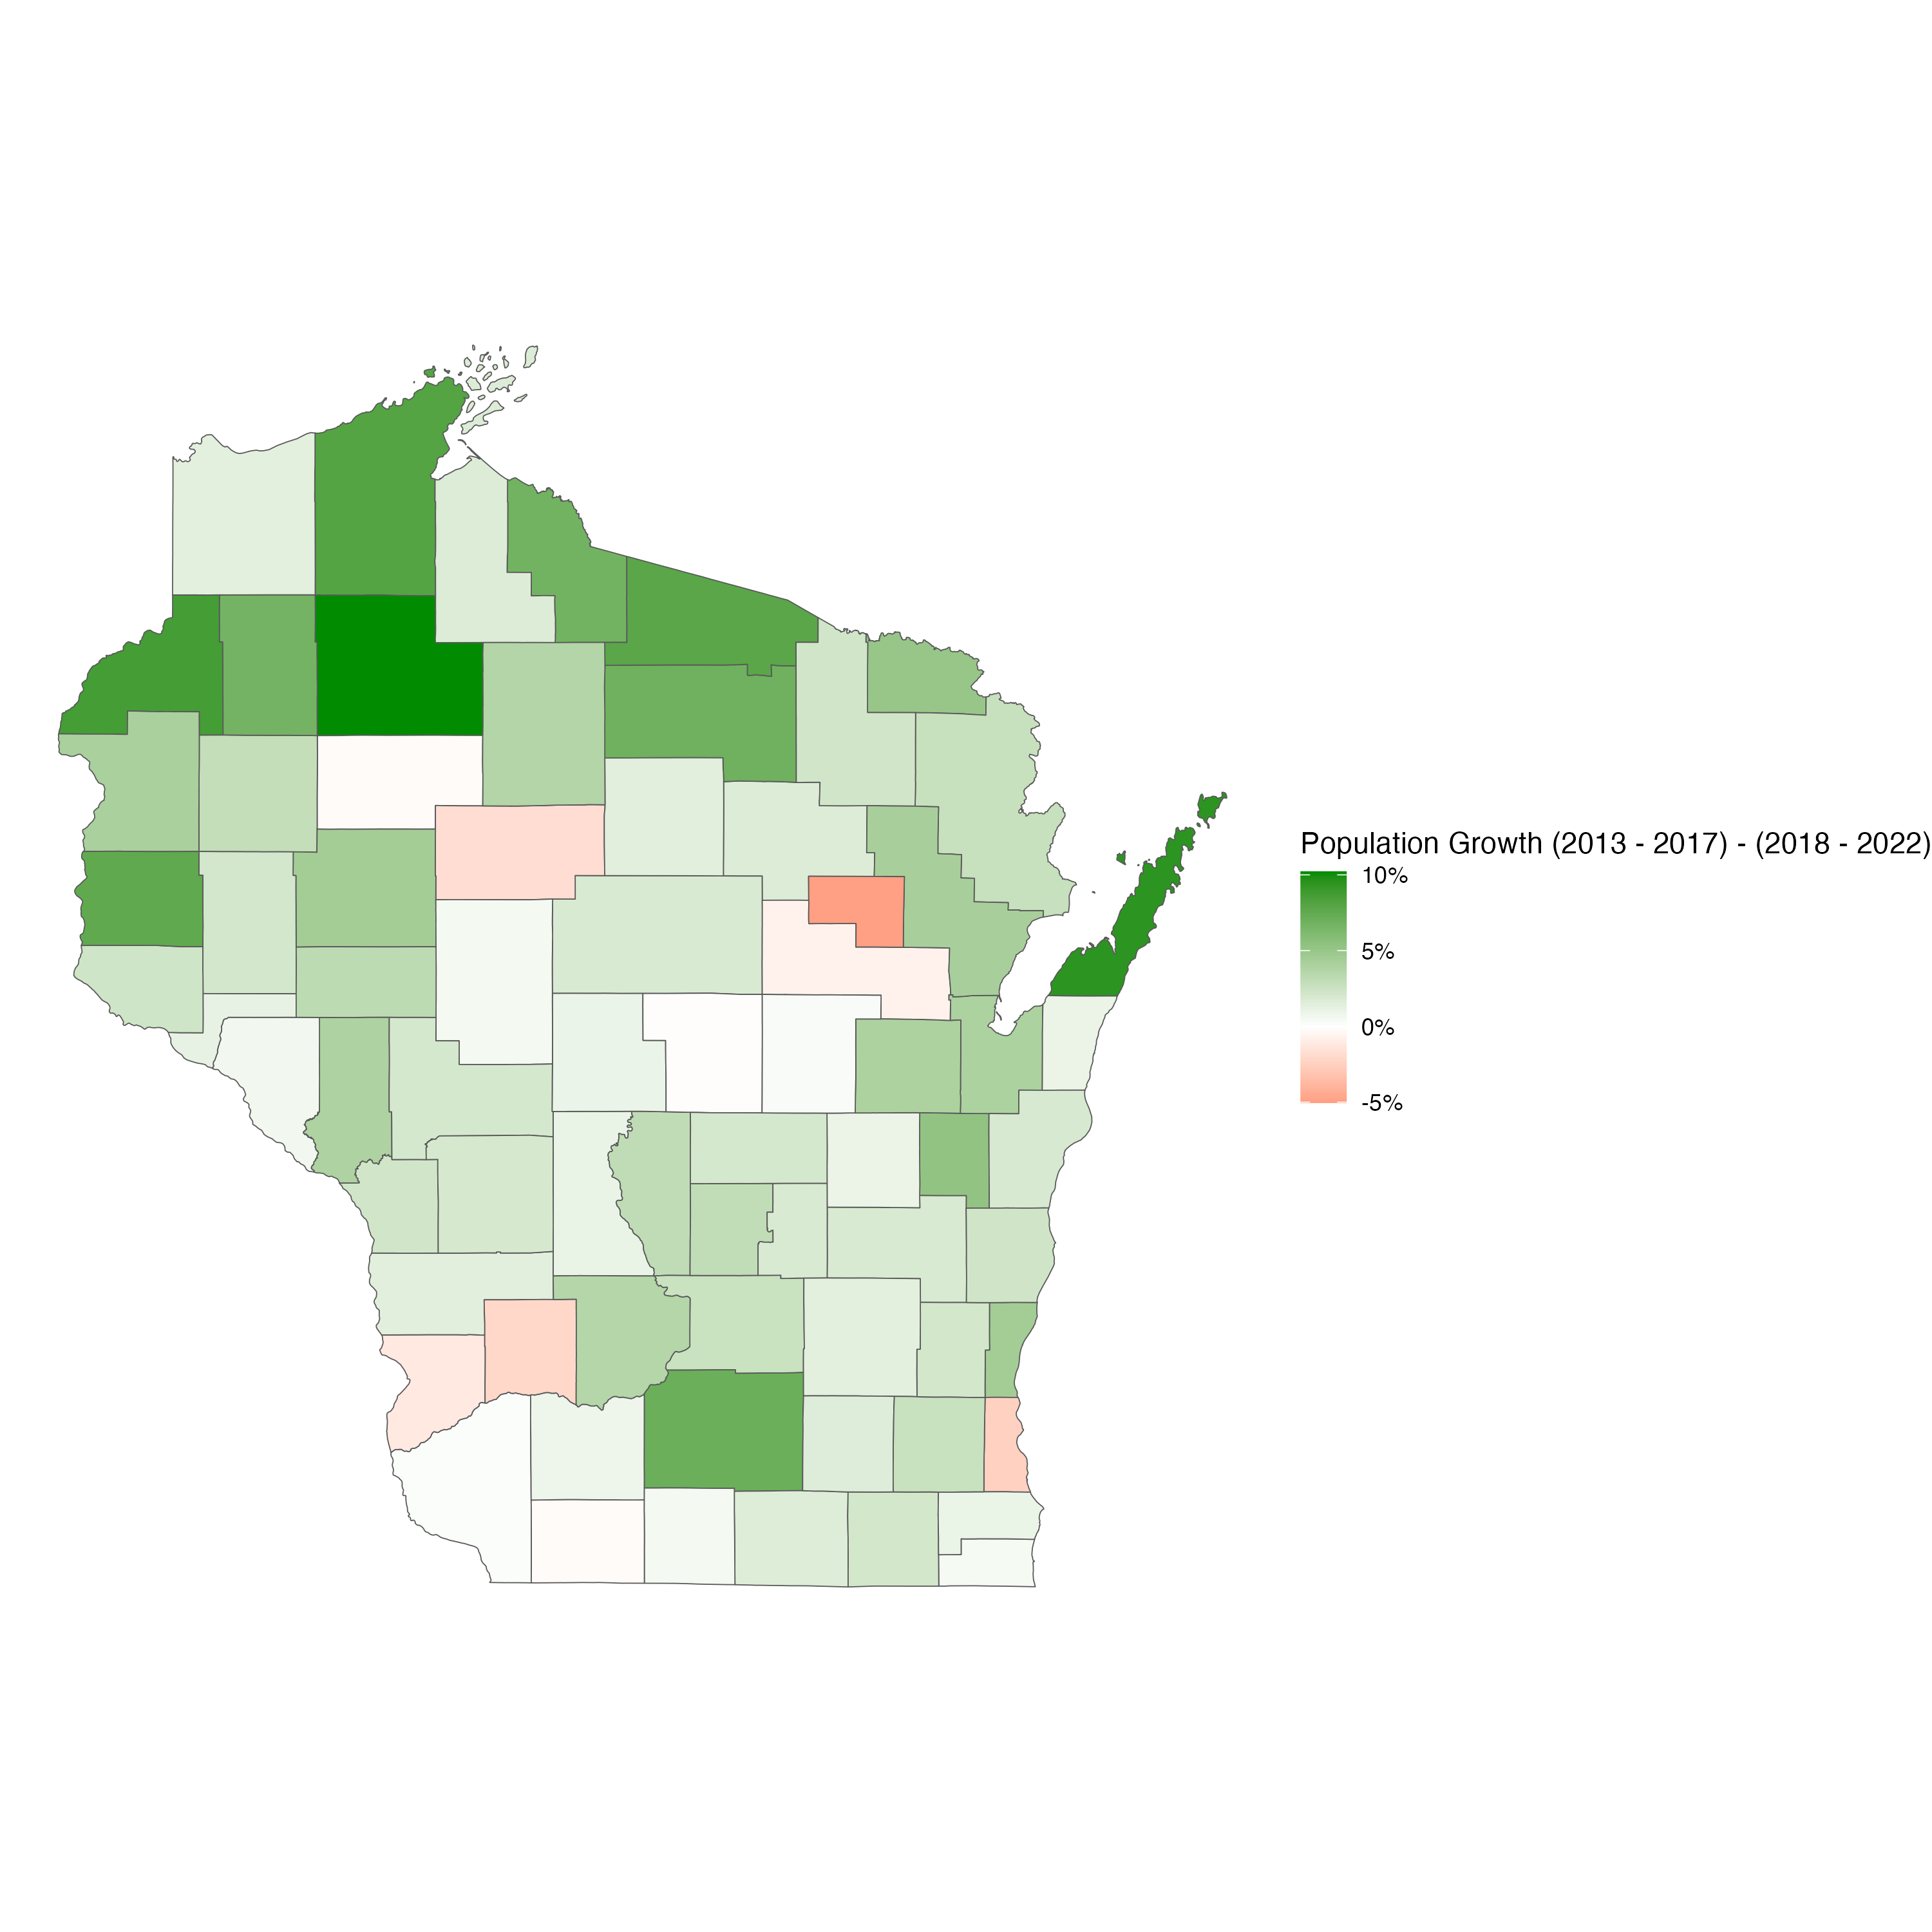
\includegraphics[width=0.9\textwidth]{plots/wi-growth.png}
    \caption{Wisconsin: County level population growth from the 2017 ACS to the 2022 ACS}
\end{figure}
\begin{figure}
   \centering
   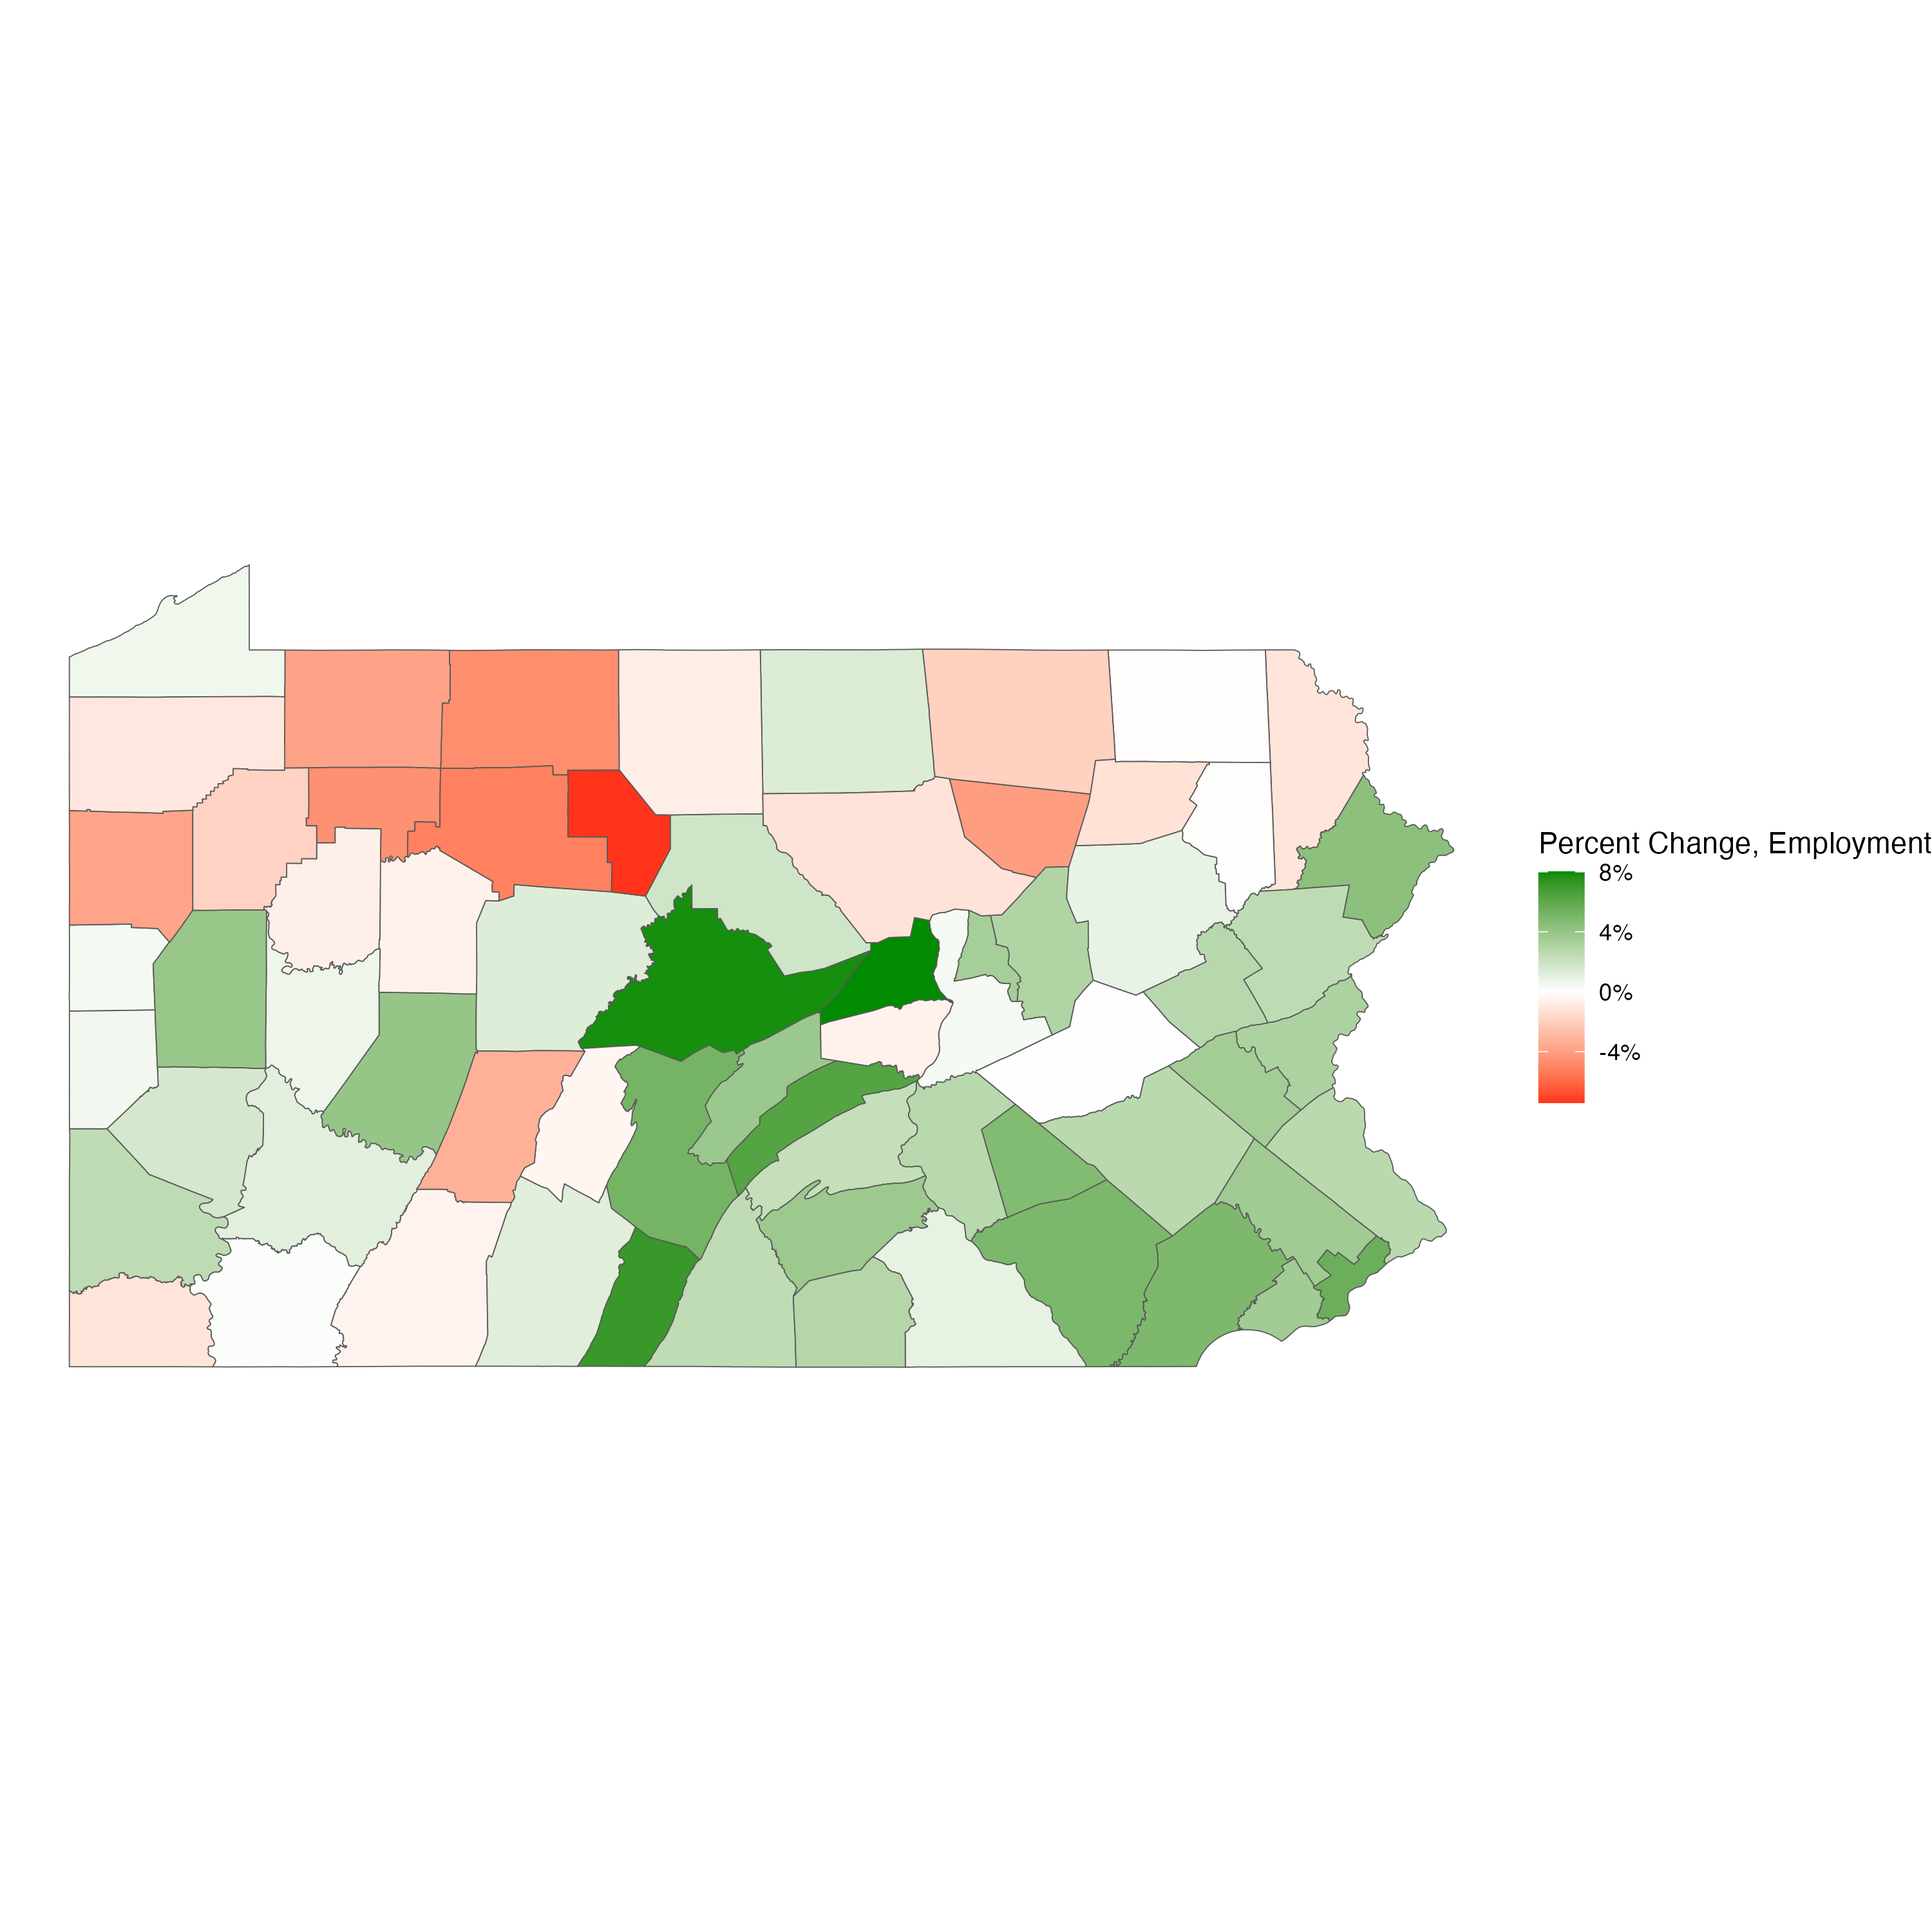
\includegraphics[width=0.9\textwidth]{plots/raw-employment-plot-pa.png}
   \caption{Pennsylvania: The percent change in the number of employed workers in each County from Trump's inauguration to February 2020, the Month before the pandemic hit}
\end{figure}
\begin{figure}
    \centering
    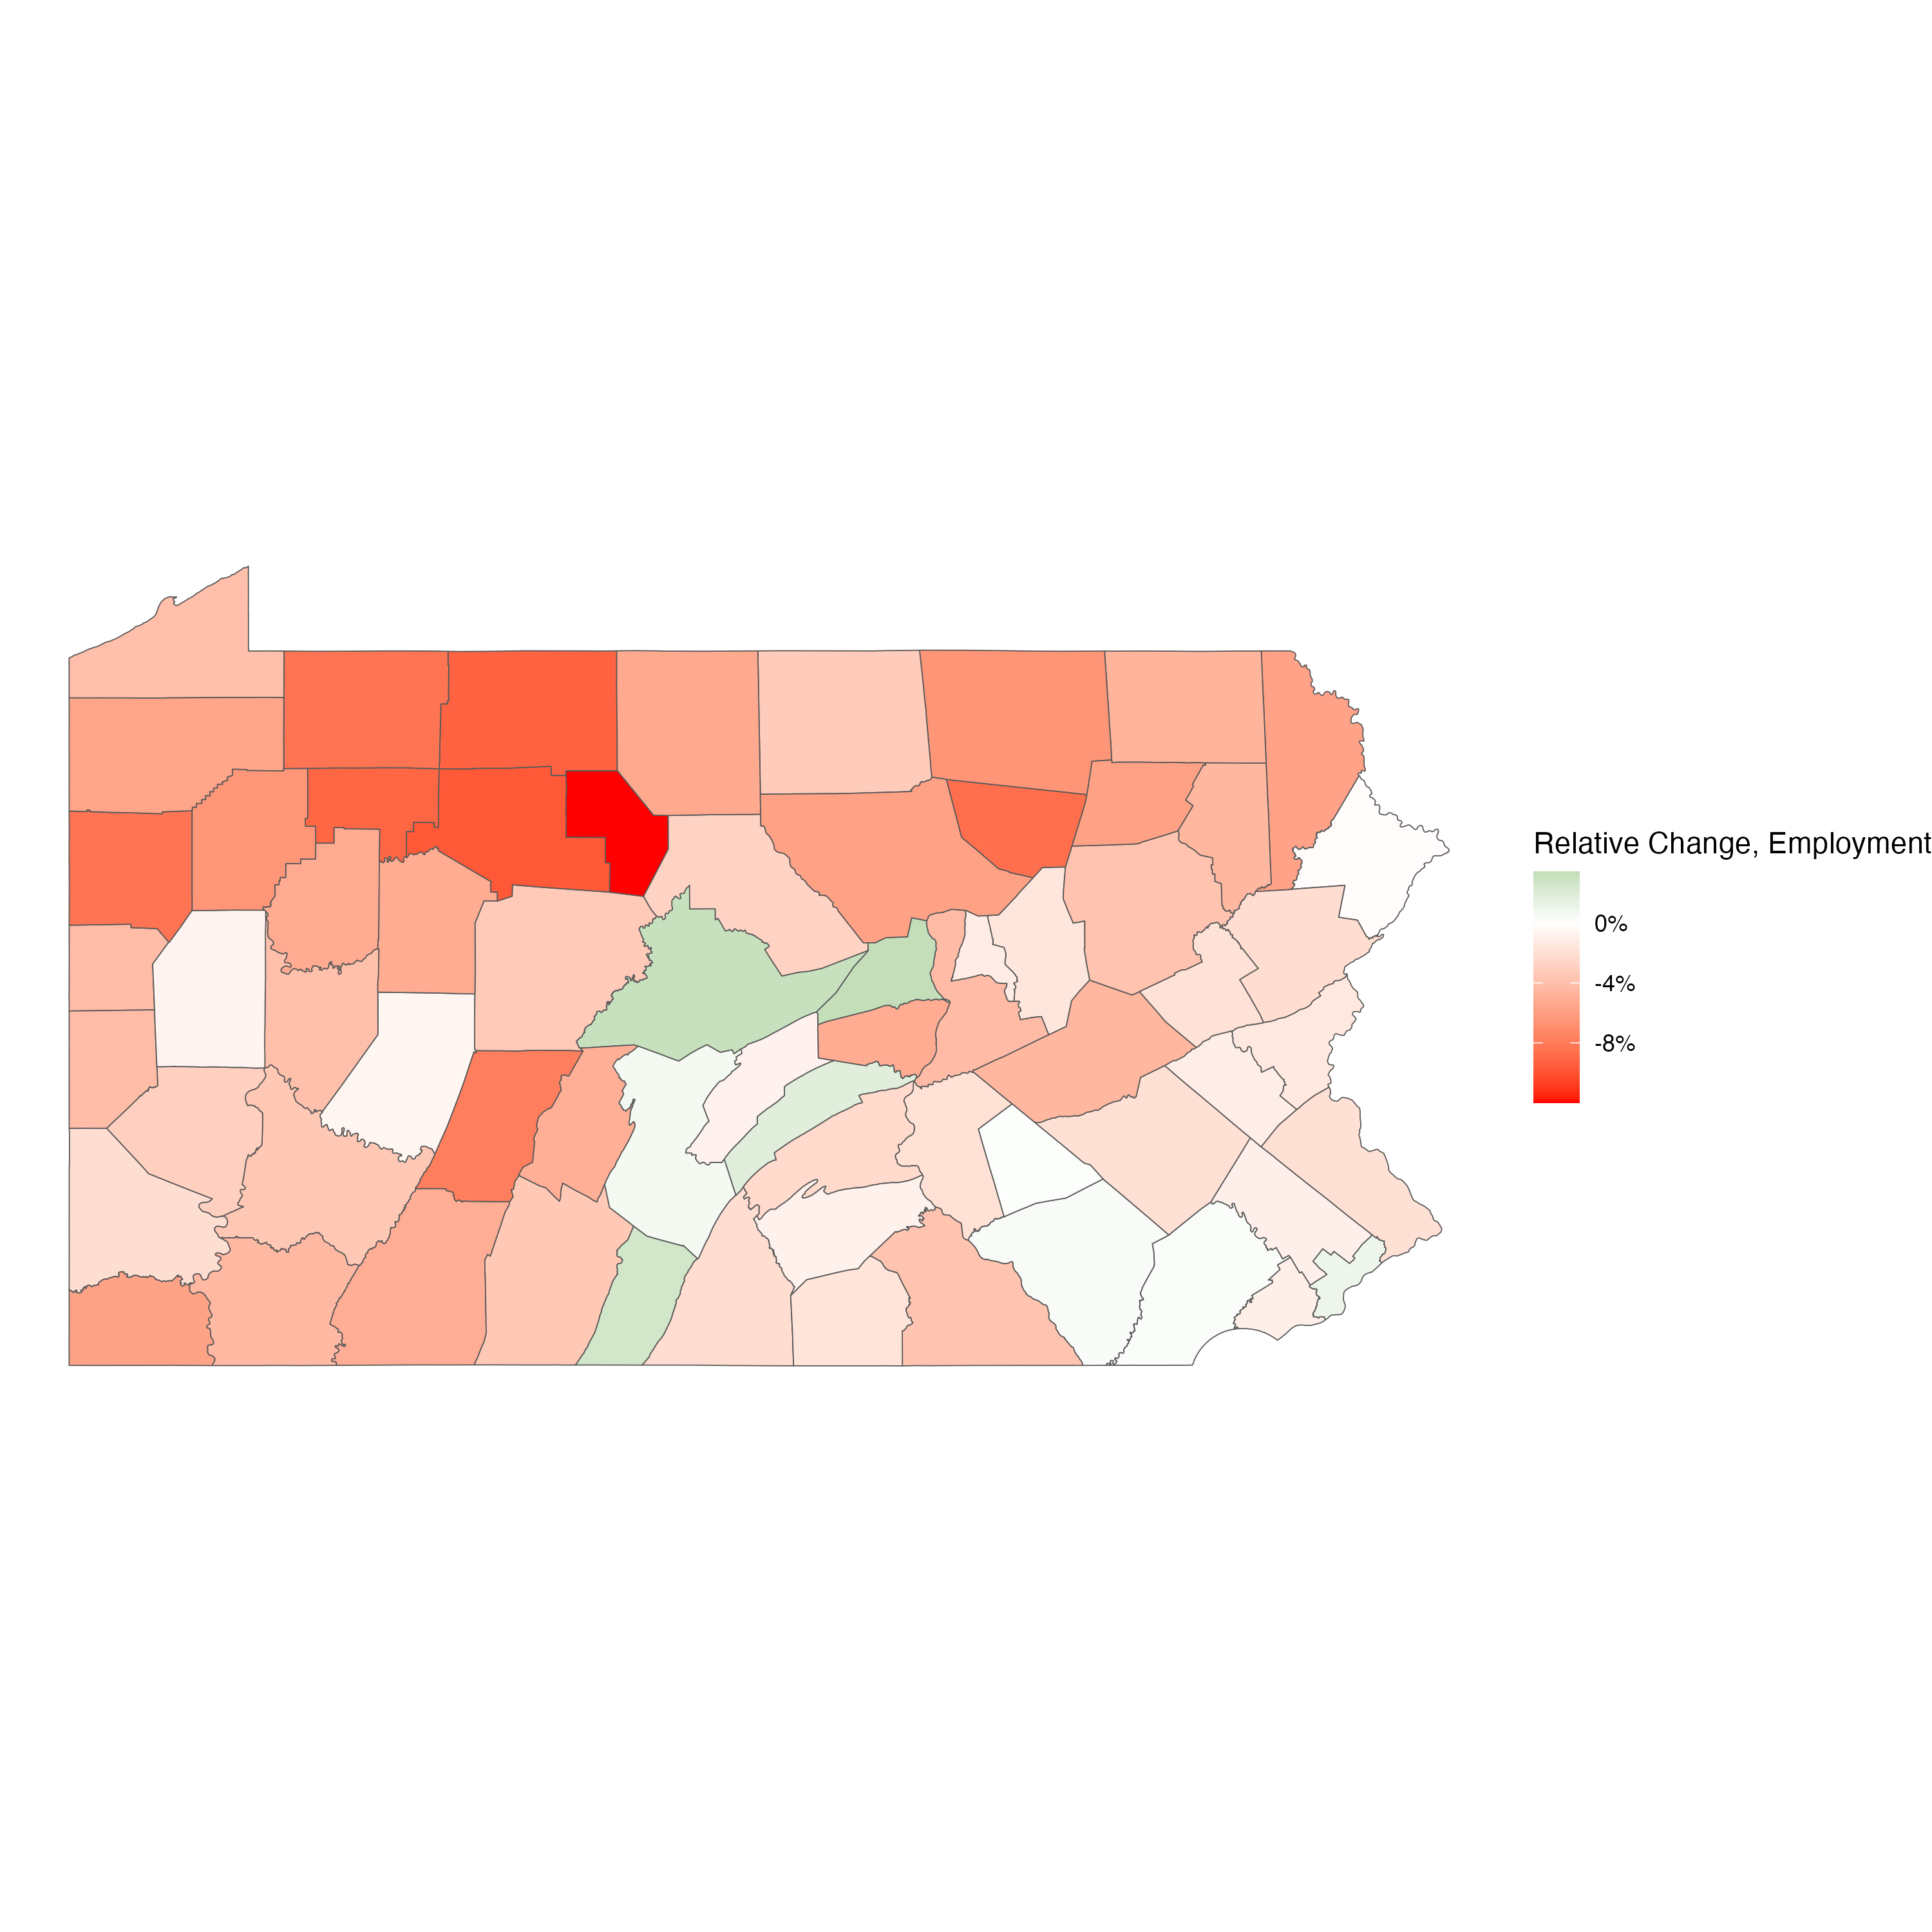
\includegraphics[width=0.9\textwidth]{plots/relative-employment-plot-pa.png}
    \caption{The percent change in the number of employed workers in each county in Pennsylvania minus the national percent change in the number of percent workers over the period from Trump's inauguration to February 2020}
\end{figure}
\begin{figure}
    \centering
    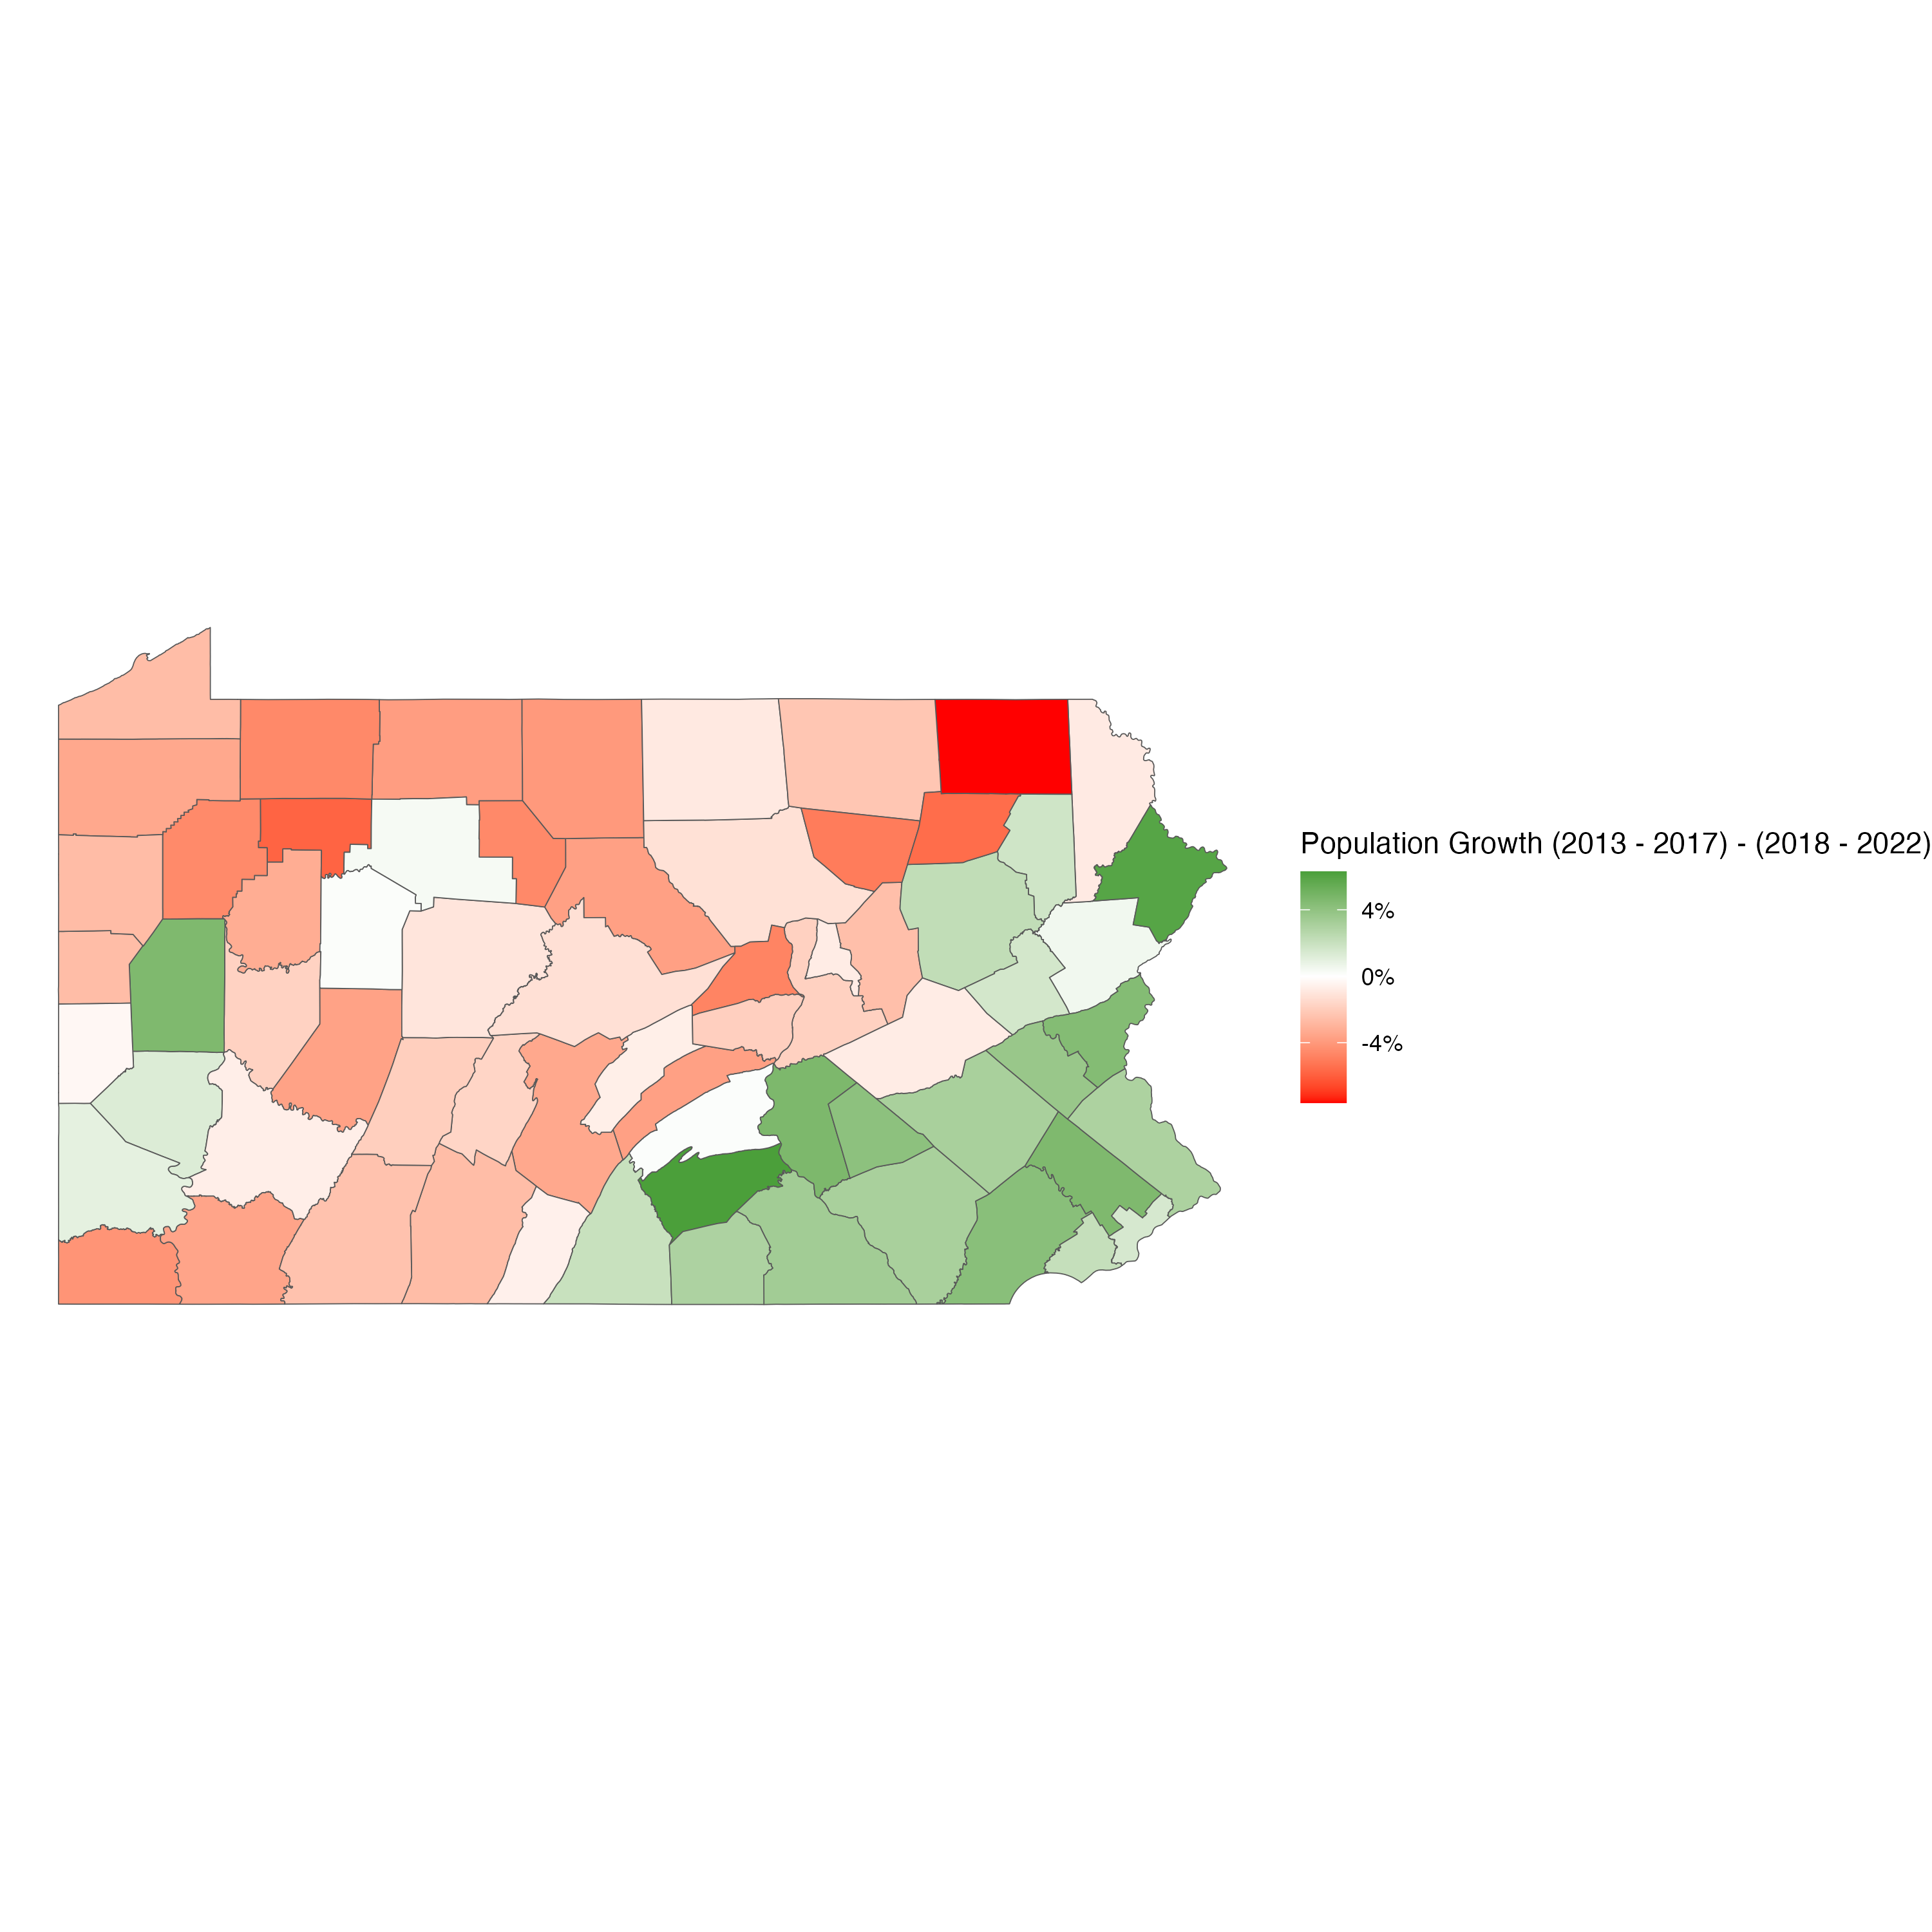
\includegraphics[width=0.9\textwidth]{plots/pa-growth.png}
    \caption{Pennsylvania: County level population growth from the 2017 ACS to the 2022 ACS}
\end{figure}
\begin{figure}
   \centering
   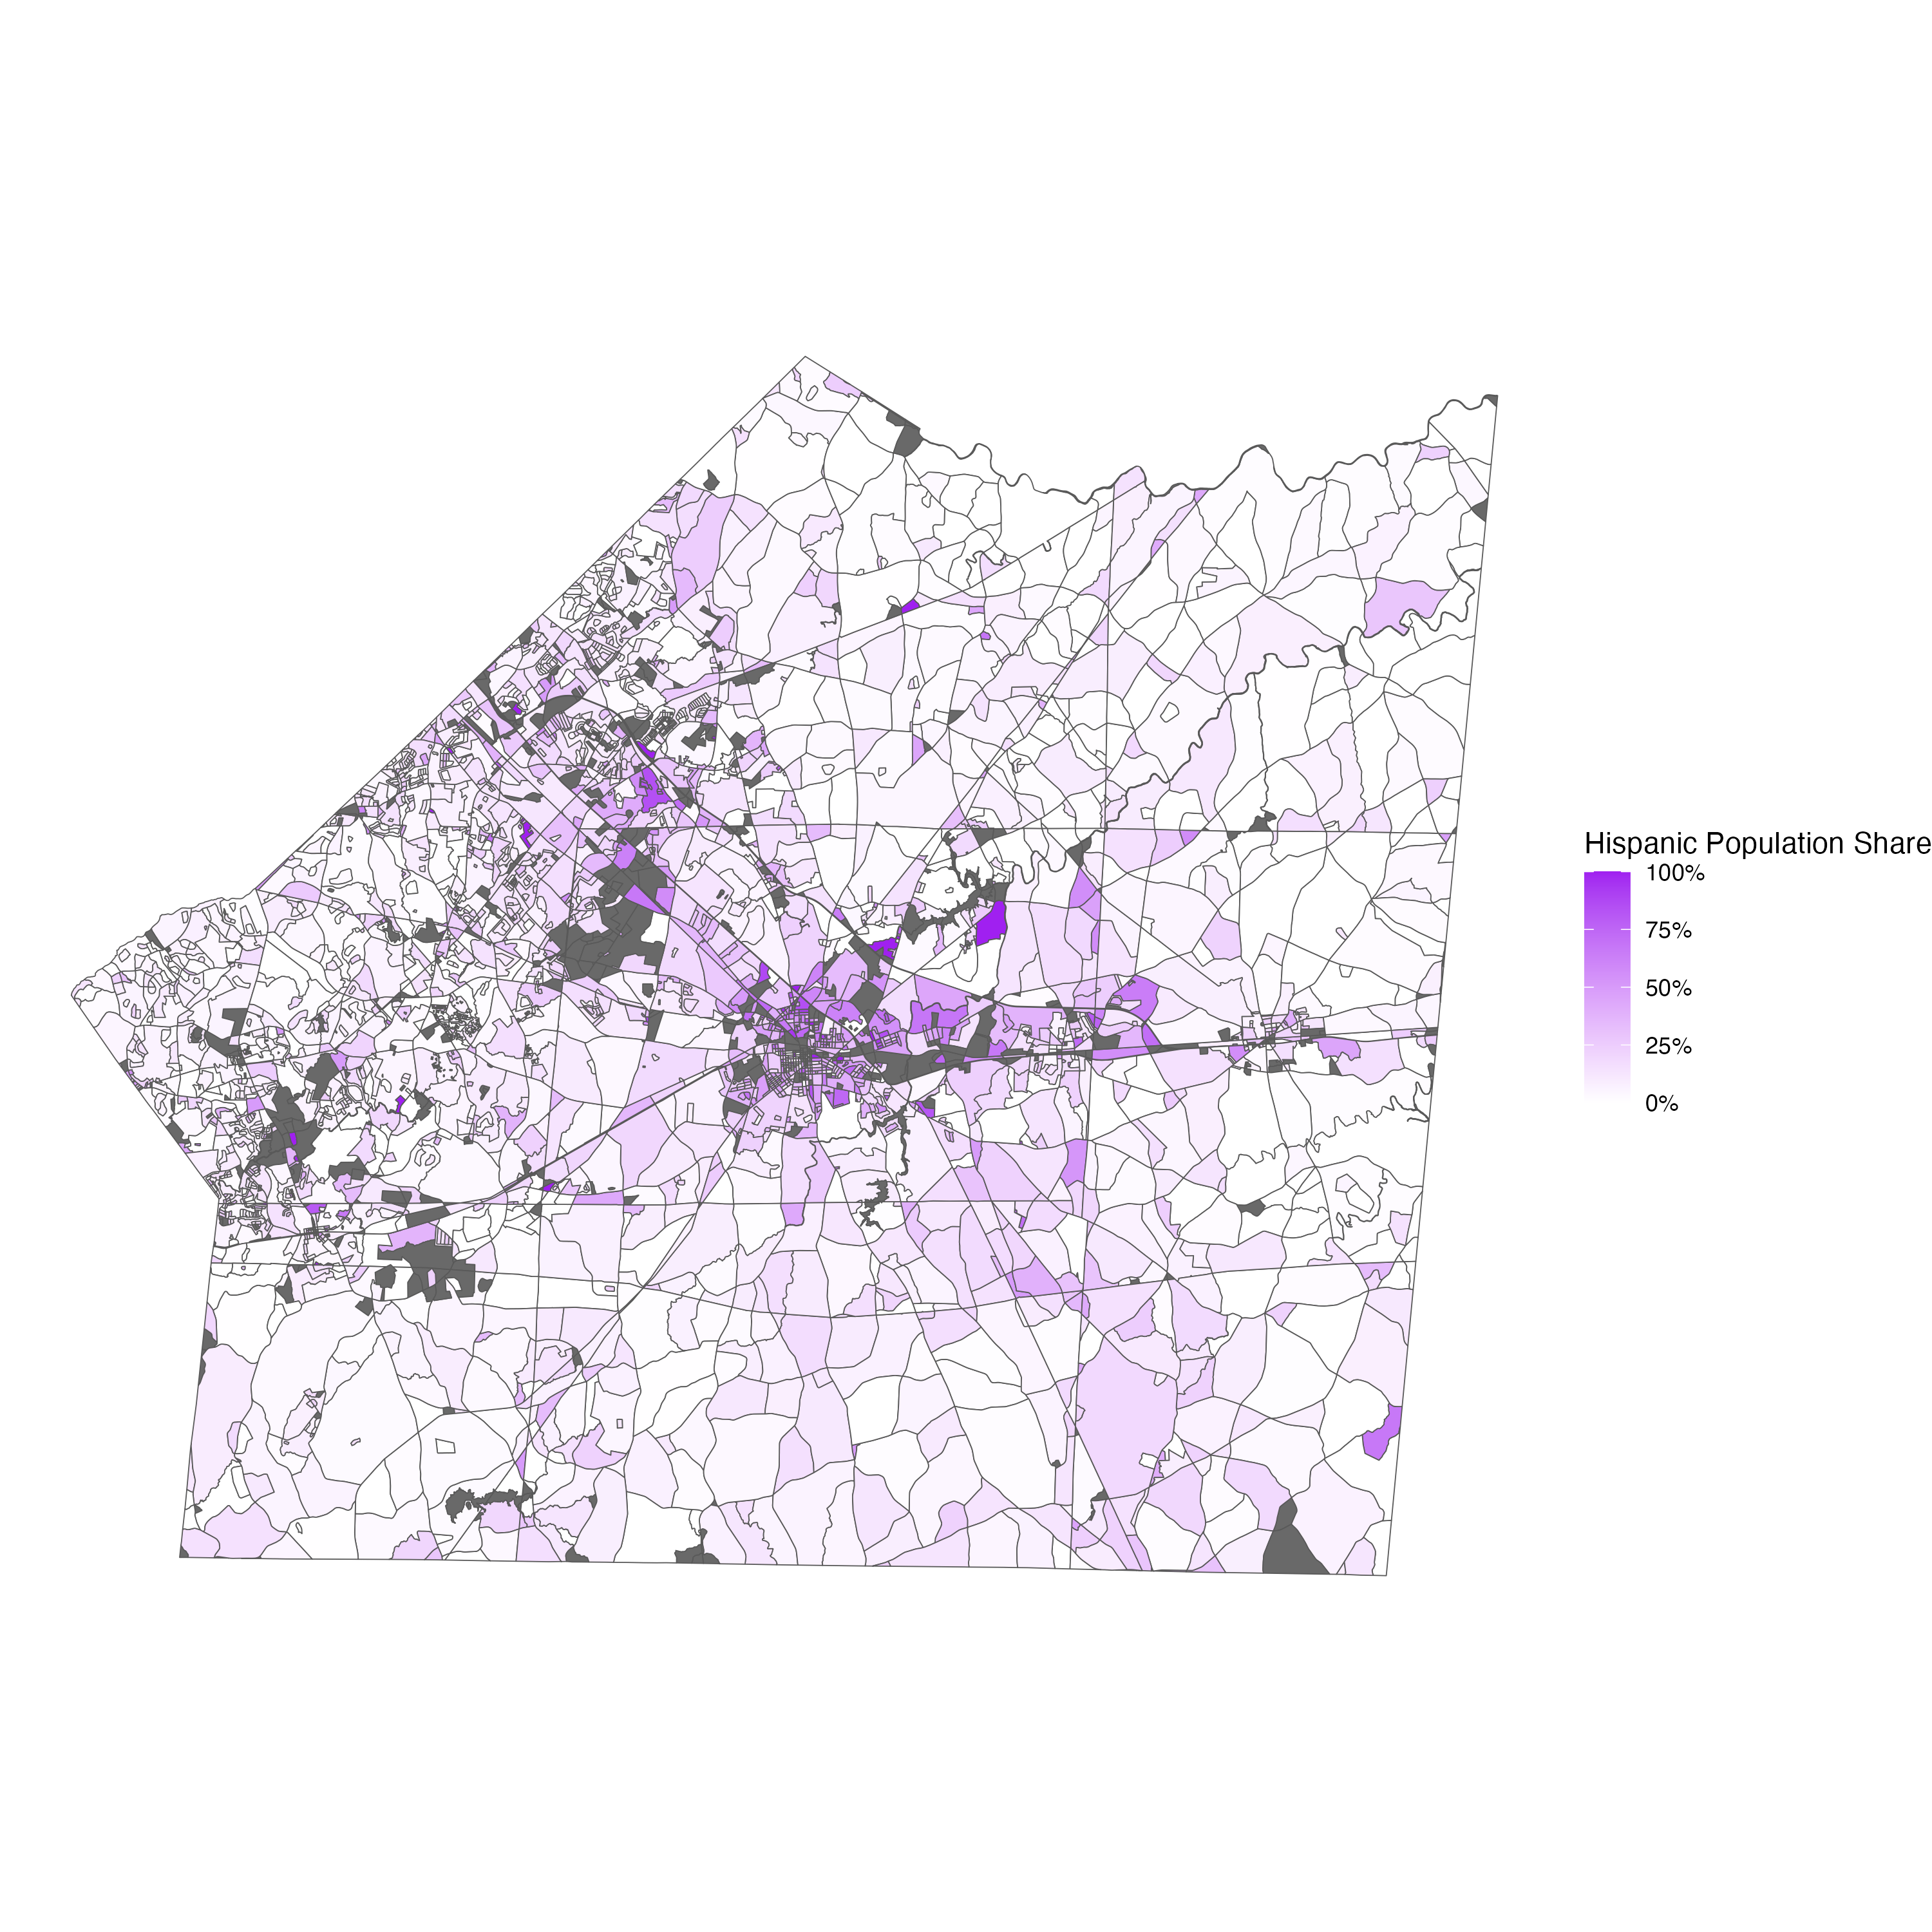
\includegraphics[width=0.9\textwidth]{plots/union_nc.png}
   \caption{2020 Census: Hispanic Population Share by block in Union County, NC}
\end{figure}
\begin{figure}
    \centering
    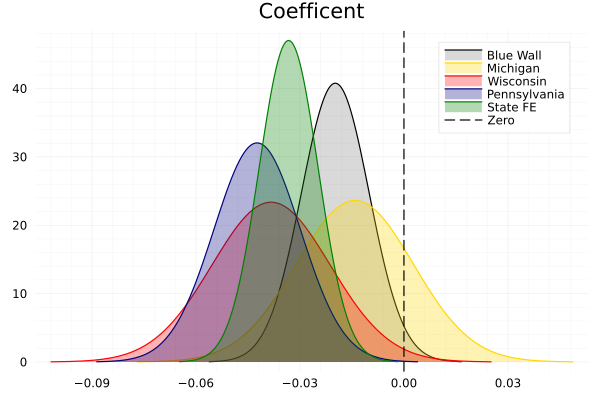
\includegraphics[width=0.45\textwidth]{plots/frequentist-coefs.png}
    \hfill 
    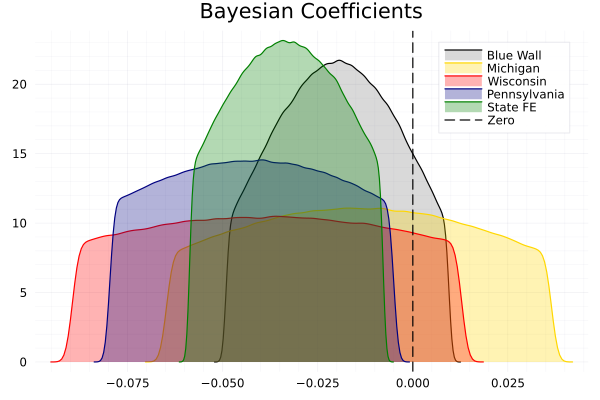
\includegraphics[width=0.45\textwidth]{plots/bayesian-corr-coefs.png}
    \caption{The distribution of the regression coefficient of county-level relative employment growth on Trump's 2016 margin. Each state individually, all three states together, and all three states together with state-level fixed effects. Frequentist Estimation on the left, Bayesian on the right.}
\end{figure}
\begin{figure}
    \centering
    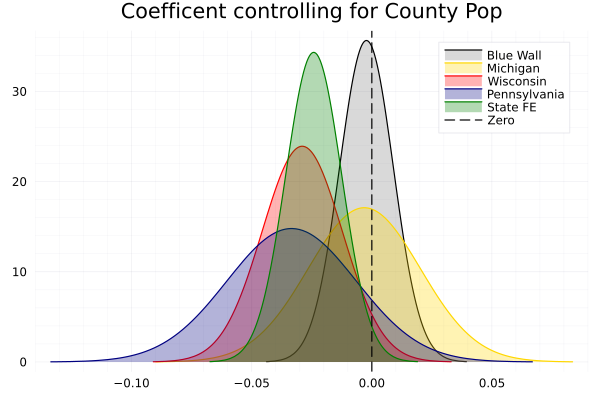
\includegraphics[width=0.45\textwidth]{plots/population-coefs.png}
    \hfill
    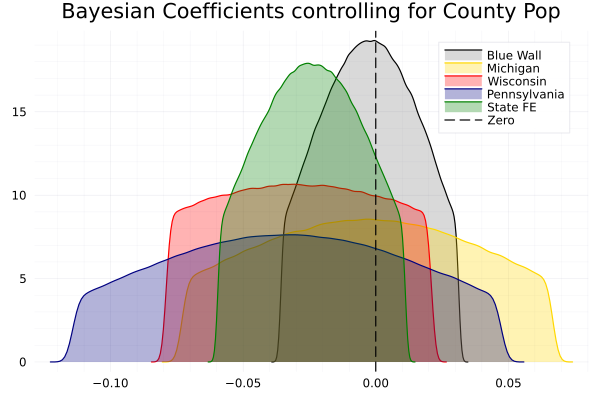
\includegraphics[width=0.45\textwidth]{plots/bayesian-pop-coefs.png}
    \caption{The distribution of the regression coefficient of county-level employment growth on Trump's 2016 margin, controlling for county-level population. Each state individually, all three states together, and all three states together with state-level fixed effects. Frequentist Estimation on the left, Bayesian on the right.}
\end{figure}
\begin{table}
    \centering
    \begin{tabular}{l|rrrr}
\toprule
                    &       \multicolumn{4}{c}{Relative County Employment Change}      \\ 
                    \hline
                    &        (1) &        (2) &        (3) &      (4) \\ 
(Intercept)         & -0.0305*** & -0.0384*** &            &          \\ 
                    &    (0.003) &    (0.004) &            &          \\ 
Trump 2016 Margin              &   -0.0198* &    -0.0022 & -0.0333*** & -0.0242* \\ 
                    &    (0.010) &    (0.011) &    (0.008) &  (0.012) \\ 
2017 County Population           &            &  0.0000*** &            &  0.0000* \\ 
                    &            &    (0.000) &            &  (0.000) \\ 
\hline
State FE &            &            &        Yes &      Yes \\ 
\hline
$R^2$               &      0.019 &      0.052 &      0.222 &    0.227 \\ 
Adjusted $R^2$      &      0.014 &      0.044 &      0.211 &    0.212 \\ 
\hline
Paradigm & \multicolumn{4}{c}{Frequentist} \\
\end{tabular}
\caption{Estimating the effect of Trump's 2016 margin on county-level employment growth from January 2017 to February 2020 in Michigan, Wisconsin, and Pennsylvania.}
\label{tab:freq}
\end{table}
\end{document}
